\section{Двумерные поверхности в трёхмерном пространстве}

\epigraph{Это яма, вырытая для нас великими предшественниками.}{А.\,А. Гайфуллин}

\subsection{Криволинейные системы координат в $\R^n$}

Рассмотрим область $U$ пространства $\R^n$ с декартовыми координатами $(x^1, \ldots, x^n)$. Предположим, что в другом экземпляре пространства $\R^n$ с координатами $(u^1, \ldots, u^n)$ задана область $V$ и установлено взаимно однозначное соответствие между точками областей $U$ и $V$. В этом случае для задания точки области $U$ мы можем использовать набор чисел $(u^1, \ldots, u^n)$ --- декартовы координаты соответствующей точки в области $V$.

\begin{definition}
	Будем говорить, что $(u^1, \ldots, u^n)$ являются \textit{криволинейными координатами} в области $U$, если:
	\begin{enumerate}[nolistsep, label=(\arabic*)]
		\item функции
			\[
				x^i = x^i(u^1, \ldots, u^n),
			\]
			задающие биекцию между областями $U$ и $V$, достаточно гладкие в области $V$;
		\item якобиан $\ds J = \det\br{\frac{\partial x^i}{\partial u^j}}$ отличен от нуля в области $V$ (условие регулярности);
	\end{enumerate}
\end{definition}

По теореме об обратной функции (якобиан не равен нулю) существуют достаточно гладкие обратные отображения $u^i = u^i(x^1, \ldots, x^n)$, причём якобиан $\ds\widetilde{J} = \det\br{\frac{\partial u^i}{\partial x^j}}$ отличен от нуля (он равен $J^{-1}$).

В области $U$ условия $u^i = \const$ определяют $n$ семейств \textit{координатных гиперповерхностей}. (Координатные гиперповерхности одного и того же семейства не пересекаются.)

Любые $n - 1$ координатных гиперповерхностей, принадлежащих различным семействам, пересекаются по некоторой кривой. Такие кривые называют \textit{координатными линиями}.

\begin{definition}
	Система криволинейных координат, вектора скорости координатных линий которой перпендикулярны друг другу, называется \textit{ортогональной}.
\end{definition}

\begin{problem}
	Для эллипсоидальной системы координат, определяемой равенствами
	\begin{gather*}
		x_1^2 = \frac{(a_1 - u_1)(a_1 - u_2)(a_1 - u_3)}{(a_2 - a_1)(a_3 - a_1)},\\
		x_2^2 = \frac{(a_2 - u_1)(a_2 - u_2)(a_2 - u_3)}{(a_3 - a_2)(a_1 - a_2)},\\
		x_3^2 = \frac{(a_3 - u_1)(a_3 - u_2)(a_3 - u_3)}{(a_1 - a_3)(a_2 - a_3)},
	\end{gather*}
	где $a_1 > a_2 > a_3 > 0$, $u_1 < a_3 < u_2 < a_2 < u_3 < a_1$,
	\begin{enumerate}[nolistsep, label=(\arabic*)]
		\item найти координатные поверхности и координатные линии;
		\item посчитать определители $\ds\det\br{\frac{\partial x_i}{\partial u_j}}$ и $\ds\det\br{\frac{\partial u_i}{\partial x_j}}$ и установить, в каких точках пространства $\R^3$ нарушается взаимная однозначность соответствия между криволинейными и прямоугольными декартовыми координатами;
		\item определить, является ли эта система координат ортогональной.
	\end{enumerate}
\end{problem}

\begin{solution}
	\begin{enumerate}[nolistsep, label=(\arabic*)]
		\item Фиксируем $u_1 = \lambda$. Тогда
			\begin{multline*}
				\frac{x_1^2}{a_1 - \lambda} + \frac{x_2^2}{a_2 - \lambda} + \frac{x_3^2}{a_3 - \lambda} = \frac{(a_1 - u_2)(a_1 - u_3)}{(a_2 - a_1)(a_3 - a_1)} + \frac{(a_2 - u_2)(a_2 - u_3)}{(a_3 - a_2)(a_1 - a_2)} + {}\\{} + \frac{(a_3 - u_2)(a_3 - u_3)}{(a_1 - a_3)(a_2 - a_3)} = \frac{1}{(a_1 - a_2)(a_2 - a_3)(a_3 - a_1)}\Big((a_3 - a_2)(a_1 - u_2)(a_1 - u_3) + {}\\{} + (a_1 - a_3)(a_2 - u_2)(a_2 - u_3) + (a_2 - a_1)(a_3 - u_2)(a_3 - u_3)\Big) = \varphi(u_2, u_3).
			\end{multline*}

			При этом $\varphi = Au_2 + Bu_3 + Cu_2u_3 + D$. Нетрудно убедиться, что все коэффициенты, кроме $D$, нулевые, а $D$ равен $1$. Например, для коэффициента при $u_2$ имеем
			\begin{multline*}
				(\ldots) \cdot A = (a_1a_2 - a_1a_3) + (a_2a_3 - a_1a_2) + (a_1a_3 - a_2a_3) = \\= \cancel{(a_1a_2 - a_1a_2)} + \cancel{(a_2a_3 - a_2a_3)} + \cancel{(a_3a_1 - a_3a_1)} = 0.
			\end{multline*}

			Отсюда, $\varphi \equiv 1$. Итак, имеем координатные поверхности
			\[
				\frac{x_1^2}{a_1 - \lambda} + \frac{x_2^2}{a_2 - \lambda} + \frac{x_3^2}{a_3 - \lambda} = 1,
			\]
			представляющие собой эллипсоиды.

			Для остальных координат всё аналогично. Фиксируя $u_2 = \mu$, получаем семейство однополостных гиперболоидов:
			\[
				\frac{x_1^2}{a_1 - \mu} + \frac{x_2^2}{a_2 - \mu} - \frac{x_3^2}{\mu - a_3} = 1.
			\]
			(Формула та же, но $a_3 < \mu$.) Для фиксированного $u_3 = \nu$ получаем семейство двуполостных гиперболоидов:
			\[
				\frac{x_1^2}{a_1 - \nu} - \frac{x_2^2}{\nu - a_2} - \frac{x_3^2}{\nu - a_3} = 1.
			\]
		\item Найдём, например, производную $\partial x_1 / \partial u_2$:
			\begin{gather*}
				x_1(u_2) = \sqrt{\frac{(a_1 - u_1)(a_1 - u_2)(a_1 - u_3)}{(a_2 - a_1)(a_3 - a_1)}} = \sqrt{\frac{(a_1 - u_1)(a_1 - u_3)}{(a_2 - a_1)(a_3 - a_1)}} \cdot \sqrt{a_1 - u_2},\\
				\frac{\partial x_1}{\partial u_2} = \sqrt{\frac{(a_1 - u_1)(a_1 - u_3)}{(a_2 - a_1)(a_3 - a_1)}} \cdot \frac{-1}{2\sqrt{a_1 - u_2}} = -\frac{1}{2}\sqrt{\frac{(a_1 - u_1)(a_1 - u_3)}{(a_2 - a_1)(a_3 - a_1)(a_1 - u_2)}}.
			\end{gather*}
			Отсюда понятен общий вид выражения $\partial x_i / \partial u_j$. Считаем определитель:
			\begin{fullwidth}
				\begin{multline*}
					\det\br{\frac{\partial x_i}{\partial u_j}} =\\ = -\frac{1}{8}\det
					\begin{pmatrix}
						\sqrt{\frac{(a_1 - u_2)(a_1 - u_3)}{(a_2 - a_1)(a_3 - a_1)(a_1 - u_1)}} & \sqrt{\frac{(a_1 - u_1)(a_1 - u_3)}{(a_2 - a_1)(a_3 - a_1)(a_1 - u_2)}} & \sqrt{\frac{(a_1 - u_1)(a_1 - u_2)}{(a_2 - a_1)(a_3 - a_1)(a_1 - u_3)}}\\
						\sqrt{\frac{(a_2 - u_2)(a_2 - u_3)}{(a_1 - a_2)(a_3 - a_2)(a_2 - u_1)}} & \sqrt{\frac{(a_2 - u_1)(a_2 - u_3)}{(a_1 - a_2)(a_3 - a_2)(a_2 - u_2)}} & \sqrt{\frac{(a_2 - u_1)(a_2 - u_2)}{(a_1 - a_2)(a_3 - a_2)(a_2 - u_3)}}\\
						\sqrt{\frac{(a_3 - u_2)(a_3 - u_3)}{(a_1 - a_3)(a_2 - a_3)(a_3 - u_1)}} & \sqrt{\frac{(a_3 - u_1)(a_3 - u_3)}{(a_1 - a_3)(a_2 - a_3)(a_3 - u_2)}} & \sqrt{\frac{(a_3 - u_1)(a_3 - u_2)}{(a_1 - a_3)(a_2 - a_3)(a_3 - u_3)}}
					\end{pmatrix} =\\ =
					\frac{1}{8} \cdot \frac{1}{(a_1 - a_2)(a_2 - a_3)(a_3 - a_1)}\det
					\begin{pmatrix}
						\sqrt{\frac{(a_1 - u_2)(a_1 - u_3)}{a_1 - u_1}} & \sqrt{\frac{(a_1 - u_1)(a_1 - u_3)}{a_1 - u_2}} & \sqrt{\frac{(a_1 - u_1)(a_1 - u_2)}{a_1 - u_3}}\\
						\sqrt{\frac{(a_2 - u_2)(a_2 - u_3)}{a_2 - u_1}} & \sqrt{\frac{(a_2 - u_1)(a_2 - u_3)}{a_2 - u_2}} & \sqrt{\frac{(a_2 - u_1)(a_2 - u_2)}{a_2 - u_3}}\\
						\sqrt{\frac{(a_3 - u_2)(a_3 - u_3)}{a_3 - u_1}} & \sqrt{\frac{(a_3 - u_1)(a_3 - u_3)}{a_3 - u_2}} & \sqrt{\frac{(a_3 - u_1)(a_3 - u_2)}{a_3 - u_3}}
					\end{pmatrix} =\\ = \frac{1}{8} \cdot \frac{1}{(a_1 - a_2)(a_2 - a_3)(a_3 - a_1)} \sqrt{-\prod_{i, j = 1}^3(a_i - u_j)} \cdot \det
					\begin{pmatrix}
						\frac{1}{a_1 - u_1} & \frac{1}{a_1 - u_2} & \frac{1}{a_1 - u_3}\\
						\frac{1}{a_2 - u_1} & \frac{1}{a_2 - u_2} & \frac{1}{a_2 - u_3}\\
						\frac{1}{a_3 - u_1} & \frac{1}{a_3 - u_2} & \frac{1}{a_3 - u_3}
					\end{pmatrix}.
				\end{multline*}
			\end{fullwidth}
			 Чтобы вычислить оставшийся определитель, вычтем первую строку из двух других:
			\begin{multline*}
				\det
				\begin{pmatrix}
					\frac{1}{a_1 - u_1} & \frac{1}{a_1 - u_2} & \frac{1}{a_1 - u_3}\\
					\frac{1}{a_2 - u_1} & \frac{1}{a_2 - u_2} & \frac{1}{a_2 - u_3}\\
					\frac{1}{a_3 - u_1} & \frac{1}{a_3 - u_2} & \frac{1}{a_3 - u_3}
				\end{pmatrix} = \det
				\begin{pmatrix}
					\frac{1}{a_1 - u_1} & \frac{1}{a_1 - u_2} & \frac{1}{a_1 - u_3}\\
					\frac{a_1 - a_2}{(a_1 - u_1)(a_2 - u_1)} & \frac{a_1 - a_2}{(a_1 - u_2)(a_2 - u_2)} & \frac{a_1 - a_2}{(a_1 - u_3)(a_2 - u_3)}\\
					\frac{a_1 - a_3}{(a_1 - u_1)(a_3 - u_1)} & \frac{a_1 - a_3}{(a_1 - u_2)(a_3 - u_2)} & \frac{a_1 - a_3}{(a_1 - u_3)(a_3 - u_3)}\\
				\end{pmatrix} = \\ = (a_1 - a_2)(a_1 - a_3) \cdot \det
				\begin{pmatrix}
					\frac{1}{a_1 - u_1} & \frac{1}{a_1 - u_2} & \frac{1}{a_1 - u_3}\\
					\frac{1}{(a_1 - u_1)(a_2 - u_1)} & \frac{1}{(a_1 - u_2)(a_2 - u_2)} & \frac{1}{(a_1 - u_3)(a_2 - u_3)}\\
					\frac{1}{(a_1 - u_1)(a_3 - u_1)} & \frac{1}{(a_1 - u_2)(a_3 - u_2)} & \frac{1}{(a_1 - u_3)(a_3 - u_3)}
				\end{pmatrix} =\\ =
				\frac{(a_1 - a_2)(a_1 - a_3)}{(a_1 - u_1)(a_1 - u_2)(a_1 - u_3)}\det
				\begin{pmatrix}
					1 & 1 & 1\\
					\frac{1}{a_2 - u_1} & \frac{1}{a_2 - u_2} & \frac{1}{a_2 - u_3}\\
					\frac{1}{a_3 - u_1} & \frac{1}{a_3 - u_2} & \frac{1}{a_3 - u_3}
				\end{pmatrix}.
			\end{multline*}
			Здесь вычтем первый столбец из двух остальных:
			\begin{multline*}
				\det\begin{pmatrix}
					1 & 1 & 1\\
					\frac{1}{a_2 - u_1} & \frac{1}{a_2 - u_2} & \frac{1}{a_2 - u_3}\\
					\frac{1}{a_3 - u_1} & \frac{1}{a_3 - u_2} & \frac{1}{a_3 - u_3}
				\end{pmatrix} = \det
				\begin{pmatrix}
					1 & 0 & 0\\
					\frac{1}{a_2 - u_1} & \frac{u_1 - u_2}{(a_2 - u_2)(a_2 - u_1)} & \frac{u_1 - u_3}{(a_2 - u_1)(a_2 - u_3)}\\
					\frac{1}{a_3 - u_1} & \frac{u_1 - u_2}{(a_3 - u_2)(a_3 - u_1)} & \frac{u_1 - u_3}{(a_3 - u_1)(a_3 - u_3)}
				\end{pmatrix} =\\ = \det
				\begin{pmatrix}
					\frac{u_1 - u_2}{(a_2 - u_2)(a_2 - u_1)} & \frac{u_1 - u_3}{(a_2 - u_1)(a_2 - u_3)}\\
					\frac{u_1 - u_2}{(a_3 - u_2)(a_3 - u_1)} & \frac{u_1 - u_3}{(a_3 - u_1)(a_3 - u_3)}
				\end{pmatrix} = \frac{(u_1 - u_2)(u_1 - u_3)}{(a_2 - u_1)(a_3 - u_1)}\det
				\begin{pmatrix}
					\frac{1}{a_2 - u_2} & \frac{1}{a_2 - u_3}\\
					\frac{1}{a_3 - u_2} & \frac{1}{a_3 - u_3}
				\end{pmatrix} =\\ =
				\frac{(u_1 - u_2)(u_1 - u_3)}{(a_2 - u_1)(a_3 - u_1)}\br{\frac{1}{(a_2 - u_2)(a_3 - u_3)} - \frac{1}{(a_3 - u_2)(a_2 - u_3)}} =\\ = \frac{(u_1 - u_2)(u_1 - u_3)(u_2 - u_3)(a_3 - a_2)}{(a_2 - u_1)(a_3 - u_1)(a_2 - u_2)(a_3 - u_3)(a_3 - u_2)(a_2 - u_3)}.
			\end{multline*}

			Подставляем результат в промежуточную формулу:
			\[
				\frac{(a_1 - a_2)(a_2 - a_3)(a_3 - a_1)}{-\prod\limits_{i, j = 1}^3(a_i - u_j)}(u_1 - u_2)(u_2 - u_3)(u_3 - u_1).
			\]
			И, наконец, пишем ответ:
			\[
				\det\br{\frac{\partial x_i}{\partial u_j}} =
				\frac{(u_1 - u_2)(u_2 - u_3)(u_3 - u_1)}{8\sqrt{-\prod\limits_{i, j = 1}^3(a_i - u_j)}}.
			\]

			Взаимная однозначность координат нарушается в точках, где якобиан равен $0$. Как видно из выведенной нами формулы, это происходит при $u_i = u_j$ (для каких-то $i \ne j$). Однако по условию $u_1 < u_2 < u_3$, так что в выбранной области эллипсоидальные координаты взаимно однозначны.
		\item Из полученных уравнений координатных поверхностей видно, что они образуют квадрики, являющиеся телами вращения софокусных эллипсов и гипербол. А как известно из курса аналитической геометрии, софокусные эллипс и гипербола перпендикулярны друг другу. (А софокусные друг другу эллипсы не пересекаются, как и софокусные друг другу гиперболы.) Значит, и координатные линии, получающиеся как пересечения таких координатных поверхностей, перпендикулярны друг другу. Так что данная система координат является ортогональной.
	\end{enumerate}
\end{solution}

\begin{problem}
	Преобразовать \textit{оператор Лапласа} $\Delta V \vcentcolon = \ds\frac{\partial^2V}{\partial x^2} + \frac{\partial^2V}{\partial y^2}$ к полярным координатам $x = \rho\cos\varphi$, $y = \rho\sin\varphi$.
\end{problem}

\begin{solution}
	Формулы перехода от декартовых координат к полярным имеют вид
	\[
		\rho = \sqrt{x^2 + y^2},\quad \tg\varphi = \frac{y}{x}.
	\]
	Выражаем частные производные первого порядка:
	\[
		\frac{\partial V}{\partial x} = \frac{\partial V}{\partial \rho}\frac{\partial\rho}{\partial x} + \frac{\partial V}{\partial \varphi}\frac{\partial \varphi}{\partial x}.
	\]
	Здесь $V^\prime_\rho$ и $V^\prime_\varphi$ --- то, что нам нужно. Осталось выразить частные производные $\rho^\prime_x$ и $\varphi^\prime_x$.
	\[
		\frac{\partial\rho}{\partial x} = (\sqrt{x^2 + y^2})^\prime_x = \frac{x}{\sqrt{x^2 + y^2}} = \frac{\cancel{r}\cos\varphi}{\cancel{r}} = \cos\varphi.
	\]

	Отметим, что для вычисления $\varphi^\prime_x$ нельзя просто взять $\arctg$ от обеих частей выражения $\tg\varphi = y / x$, ведь $\varphi$ меняется от $0$ до $2\pi$, а областью значений функции $\arctg$ является интервал $\br{-\frac{\pi}{2}; \frac{\pi}{2}}$. Вместо этого выражение можно продифференцировать (по $x$):
	\[\begin{tikzcd}
		{\displaystyle\frac{1}{\cos^2\varphi}\frac{\partial\varphi}{\partial x}} & {\displaystyle\frac{\partial}{\partial x}(\tg\varphi)} & {\displaystyle\frac{\partial}{\partial x}\left(\frac{y}{x}\right) = -\frac{y}{x^2}}.
		\arrow[equals, from=1-2, to=1-1]
		\arrow[equals, from=1-2, to=1-3]
	\end{tikzcd}\]
	Отсюда находим $\displaystyle\frac{\partial\varphi}{\partial x} = -\frac{y}{x^2}\cos^2\varphi = -\frac{\sin\varphi}{\rho}$. Итого,
	\[
		\frac{\partial V}{\partial x} = \frac{\partial V}{\partial \rho}\cos\varphi - \frac{\partial V}{\partial \varphi} \frac{\sin\varphi}{\rho}.
	\]
	Аналогично находим
	\[
		\frac{\partial V}{\partial y} = \frac{\partial V}{\partial\rho}\frac{\cos\varphi}{\rho} + \frac{\partial V}{\partial \varphi}\sin\varphi.
	\]
	Переходим к нахождению вторых производных.
	\begin{multline*}
		\frac{\partial^2V}{\partial x^2} = \frac{\partial}{\partial x}\br{\frac{\partial V}{\partial x}} = \frac{\partial}{\partial\rho}\br{\frac{\partial V}{\partial x}} \cdot \frac{\partial\rho}{\partial x} + \frac{\partial}{\partial\varphi}\br{\frac{\partial V}{\partial x}} \cdot \frac{\partial\varphi}{\partial x} =\\ = \br{\frac{\partial^2V}{\partial\rho^2}\cos\varphi - \frac{\partial^2V}{\partial\varphi\partial\rho}\frac{\sin\varphi}{\rho} + \frac{\partial V}{\partial\varphi}\frac{\sin\varphi}{\rho^2}} \cdot \cos\varphi + {}\\{} + \br{\frac{\partial^2 V}{\partial\rho\partial\varphi}\cos\varphi - \frac{\partial V}{\partial\rho}\sin\varphi - \frac{\partial^2V}{\partial\varphi^2}\frac{\sin\varphi}{\rho} - \frac{\partial V}{\partial\varphi}\frac{\cos\varphi}{\rho}} \cdot \br{-\frac{\sin\varphi}{\rho}}.
	\end{multline*}
	Раскрывая скобки, получаем
	\[
		\frac{\partial^2V}{\partial x^2} = \frac{\partial^2V}{\partial\rho^2}\cos^2\varphi - \frac{\partial^2V}{\partial\rho\partial\varphi}\frac{\sin 2\varphi}{\rho} + \frac{\partial^2V}{\partial\varphi^2}\frac{\sin^2\varphi}{\rho^2} + \frac{\partial V}{\partial\varphi}\frac{\sin 2\varphi}{\rho^2} + \frac{\partial V}{\partial\rho}\frac{\sin^2\varphi}{\rho}.
	\]
	Аналогично находим
	\[
		\frac{\partial^2V}{\partial y^2} = \frac{\partial^2 V}{\partial\rho^2}\sin^2\varphi + \frac{\partial^2V}{\partial\rho\partial\varphi}\frac{\sin 2\varphi}{\rho} + \frac{\partial^2V}{\partial\varphi^2}\frac{\cos^2\varphi}{\rho^2} + \frac{\partial V}{\partial\rho}\frac{\cos^2\varphi}{\rho} - \frac{\partial V}{\partial\varphi}\frac{\sin 2\varphi}{\rho^2}.
	\]
	Полученные выражения нужно сложить:
	\begin{multline*}
		\Delta V = \frac{\partial V}{\partial x^2} + \frac{\partial V}{\partial y^2} = \frac{\partial^2 V}{\partial\rho^2}\underbrace{(\cos^2\varphi + \sin^2\varphi)}_{1} + \frac{\partial^2V}{\partial\varphi^2}\underbrace{\br{\frac{\sin^2\varphi + \cos^2\varphi}{\rho^2}}}_{1 / \rho^2} + {}\\{} + \frac{\partial V}{\partial\rho\partial\varphi}\underbrace{\br{-\frac{\sin 2\varphi}{\rho} + \frac{\sin 2\varphi}{\rho}}}_{0} + \frac{\partial V}{\partial\rho}\underbrace{\br{\frac{\sin^2\varphi + \cos^2\varphi}{\rho}}}_{1 / \rho} + \frac{\partial V}{\partial\varphi}\underbrace{\br{-2\frac{\sin 2\varphi}{\rho^2} + 2\frac{\sin 2\varphi}{\rho^2}}}_{0}.
	\end{multline*}

	\noindent
	Получаем итоговое выражение оператора Лапласа в полярных координатах:
	\[
		\Delta V = \frac{\partial^2V}{\partial\rho^2} + \frac{1}{\rho^2}\frac{\partial^2V}{\partial\varphi^2} + \frac{1}{\rho}\frac{\partial V}{\partial\rho}.
	\]
	Эту формулу часто записывают в виде
	\[
		\Delta V = \frac{1}{\rho}\frac{\partial}{\partial\rho}\br{\rho\frac{\partial V}{\partial{\rho}}} + \frac{1}{\rho^2}\frac{\partial^2V}{\partial\varphi^2}.
	\]
\end{solution}

\vspace{-.3cm}\subsection{Риманова метрика в криволинейных координатах}

Функции $x^i = x^i(u^1, \ldots, u^n)$ удобно рассматривать одновременно для всех $i = 1, \ldots, n$, используя для этого вектор-функцию
\[
	\vec{r} = \vec{r}(u^1, \ldots, u^n),\text{ где $\vec{r} = (x^1, \ldots, x^n)$}.
\]

Векторы $\vec{r}_i = \partial \vec{r} / \partial u^i$ имеют направления касательных к координатным линиям, так что в каждой точке области $U$ они линейно независимы. Они определяют в окрестности некоторой точки $(u^1, \ldots, u^n)$ малый вектор $d\vec{r} = \vec{r}_idu^i$. Квадрат его длины, выраженный в криволинейных координатах, определяет метрику:
\[
	ds^2 = \langle d\vec{r}, d\vec{r}\rangle = \left\langle\vec{r}_idu^i, \vec{r}_jdu^j\right\rangle = g_{ij}du^idu^j,
\]
где $g_{ij} = \langle\vec{r}_i, \vec{r}_j\rangle$ --- элементы матрицы Грама векторов $\vec{r}_1, \ldots, \vec{r}_n$. При переходе к другим координатам $\widetilde{u}^1, \ldots, \widetilde{u}^n$ матрица Грама преобразуется так, как и положено преобразовываться матрице квадратичной формы (по тензорному закону):
\begin{equation} \label{eq:RiemannCoordinates}
	\widetilde{g}_{ij} = \left\langle\frac{\partial \vec{r}}{\partial\widetilde{u}^i}, \frac{\partial \vec{r}}{\partial\widetilde{u}^j}\right\rangle = \left\langle\frac{\partial \vec{r}}{\partial u^k}\frac{\partial u^k}{\partial\widetilde{u}^i}, \frac{\partial \vec{r}}{\partial u^l}\frac{\partial u^l}{\partial\widetilde{u}^j}\right\rangle = \frac{\partial u^k}{\partial\widetilde{u}^i}\frac{\partial u^l}{\partial\widetilde{u}^j}g_{kl}.
\end{equation}

\begin{definition} \label{definition:RiemannMetrics}
	Говорят, что в области $U \subset \R^n$ задана \textit{риманова метрика}, если для любой криволинейной системы координат $(u^1, \ldots, u^n)$ в $U$ задана матрица $g_{ij}(u)$, которая:
	\begin{enumerate}[nolistsep, label=(\arabic*)]
		\item симметрична: $g_{ij}(u) = g_{ji}(u)$;
		\item невырожденна и положительно определена;
		\item при замене координат изменяется по формулам \eqref{eq:RiemannCoordinates}.
	\end{enumerate}
\end{definition}

\begin{problem} \label{problem:CylindricalMetric}
	Записать евклидову метрику в цилиндрической системе координат.
\end{problem}

\begin{solution}
	Запишем дифференциалы евклидовых координат:
	\begin{gather*}
		dx = d(\rho\cos\varphi) = \cos\varphi\,d\rho - \rho\sin\varphi\,d\varphi,\\
		dy = d(\rho\sin\varphi) = \sin\varphi\,d\rho + \rho\cos\varphi\,d\varphi,\\
		dz = dz.
	\end{gather*}
	Подставляем их в запись евклидовой метрики:
	\begin{multline*}
		ds^2 = dx^2 + dy^2 + dz^2 = (\cos\varphi\,d\rho - \rho\sin\varphi\,d\varphi)^2 + (\sin\varphi\,d\rho + \rho\cos\varphi\,d\varphi)^2 + dz^2 =\\ = \cos^2\varphi\,d\rho^2 - \cancel{\rho\sin(2\varphi)\,d\rho d\varphi} + \rho^2\sin^2\varphi\,d\varphi^2 + {}\\ + \rho^2\sin^2\varphi\,d\rho^2 + \cancel{\rho\sin(2\varphi)\,d\rho d\varphi} + \rho^2\cos^2\varphi\,d\varphi + dz^2 = d\rho^2 + \rho^2\,d\varphi^2 + dz^2.
	\end{multline*}
\end{solution}

Пусть имеем параметризованную кривую $\vec{r}(t)$ в криволинейных координатах $(u^1, \ldots, u^n)$ с римановой метрикой, заданной матрицей $G = g_{ij}$. Измеряем длину кривой, заметаемой при изменении параметра от $a$ до $b$:
\begin{equation} \label{eq:RiemannLength}
	l = \int\limits_a^b\abs{\frac{d\vec{r}}{dt}}dt = \int\limits_a^b\sqrt{\left\langle \frac{d\vec{r}}{dt}, \frac{d\vec{r}}{dt} \right\rangle}\,dt = \int\limits_a^b\sqrt{\frac{ds^2}{(dt)^2}}\,dt = \int\limits_a^b\sqrt{g_{ij}\frac{du^i}{dt}\frac{du^j}{dt}}\,dt.
\end{equation}

\begin{problem}
	Проверить, что матрица
	\[
		\G(u, v) = \frac{1}{1 - u^2 - v^2}
		\begin{pmatrix}
			1 - v^2 & uv\\
			uv & 1 - u^2
		\end{pmatrix}
	\]
	задаёт риманову метрику в единичном круге на плоскости с координатами $(u, v)$. Вычислить в этой метрике длину кривой $u^2 + v^2 = a^2$, где $0 < a < 1$.
\end{problem}

\begin{proof}
	Нужно проверить лишь то, что матрица $G$ невырожденна и положительно определена, для этого можно воспользоваться критерием Сильвестра. Для минора $1 \times 1$ всё очевидно, остаётся проверить знак определителя всей матрицы $2 \times 2$:
	\[
		\det\G = \frac{(1 - v^2)(1 - u^2) - u^2v^2}{1 - u^2 - v^2} = \frac{\cancel{1 - u^2 - v^2}}{\cancel{1 - u^2 - v^2}} = 1.
	\]
	
	Если параметризовать нашу кривую как $\vec{r}(t) = (u(t), v(t))$, где $u(t) = a\cos t$, $v(t) = a\sin t$ (где $t$ меняется от $0$ до $2\pi$), то длина вычисляется по формуле \eqref{eq:RiemannLength}:
	\[
		l = \int\limits_0^{2\pi}\sqrt{\begin{pmatrix}\dot{u}(t) & \dot{v}(t)\end{pmatrix} \G \begin{pmatrix}\dot{u}(t) \\ \dot{v}(t) \end{pmatrix}}\,dt.
	\]
	Подставляем:
	\begin{multline*}
		\int\limits_0^{2\pi}\sqrt{\begin{pmatrix}-a\sin t & a\cos t\end{pmatrix} \cdot \left(\frac{1}{1 - a^2}\begin{pmatrix} 1 - a^2\sin^2t & a^2\sin t\cos t \\ a^2\sin t\cos t & 1 - a^2\cos^2t \end{pmatrix}\right) \cdot \begin{pmatrix} -a\sin t \\ a\cos t \end{pmatrix}}\,dt =\\ = \int\limits_0^{2\pi}\sqrt{\begin{pmatrix} -a\sin t & a\cos t \end{pmatrix} \cdot \left(\frac{1}{\cancel{1 - a^2}}\begin{pmatrix} -a\sin t\cancel{(1 - a^2)} \\ a\cos t\cancel{(1 - a^2)}\end{pmatrix}\right)}\,dt =\\ = \int\limits_0^{2\pi}\sqrt{a^2(\cos^2t + \sin^2t)}\,dt = \int\limits_0^{2\pi}a\,dt = 2\pi a.
	\end{multline*}
\end{proof}

Правильно думать, что матрица $\G(u^1, \ldots, u^n)$ (как матрица Грама линейно независимых векторов) симметрична и положительно определена, а потому задаёт скалярное произведение (своё в каждой точке области $U \subset \R^n$). В криволинейной системе координат $(u^1, \ldots, u^n)$ мы работаем именно в этом скалярном произведении. Например, можем считать длины кривых (что уже было продемонстрировано) или углы между кривыми.

\begin{problem}
	Найти угол между кривыми $v = 2u + 1$ и $v = -2u + 1$ на плоскости с координатами $(u, v)$ с метрикой
	\[
		ds^2 = 2du^2 + 2dudv + 4dv^2.
	\]
\end{problem}

\begin{solution}
	Данная в условии метрика задаётся матрицей
	\[
		\G =
		\begin{pmatrix}
			2 & 1\\
			1 & 4
		\end{pmatrix}.
	\]

	Параметризуем обе эти кривые: $\vec{r}_1(t) = (t, 2t + 1)$, $\vec{r}_2(t) = (t, -2t + 1)$. Они пересекаются в единственной точке $(0, 1)$ при $t = 0$. Вектора скорости этих кривых в данной точке есть $\vec{v}_1 = (1, 2)$, $\vec{v}_2 = (1, -2)$. Находим угол между этими векторами по формуле:
	\[
		\cos\angle(\vec{v}_1, \vec{v}_2) = \frac{\langle\vec{v}_1, \vec{v}_2\rangle_\G}{\sqrt{\langle\vec{v}_1, \vec{v}_1\rangle_\G} \cdot \sqrt{\langle\vec{v}_2, \vec{v}_2\rangle_\G}} = \frac{-14}{\sqrt{22} \cdot \sqrt{14}} = -\sqrt{\frac{7}{11}}.
	\]
	Отсюда получаем $\angle(\vec{v}_1, \vec{v}_2) = \arccos\sqrt{\frac{7}{11}}$.
\end{solution}

\subsection{Определение поверхности. Локальные координаты}

Наиболее наглядными и интересными с геометрической точки зрения для нас будут двумерные поверхности в $\R^3$, поэтому повествование будет строиться именно вокруг них.

Мы дадим два определения поверхности: первое --- из курса О.\,И. Мохова, второе~---~из курса И.\,А. Дынникова. Определение Ивана Алексеевича, хоть и накладывает некоторые дополнительные ограничения на поверхность, оказывается более наглядным естественным (и в целом более правильным), так что дальше мы будем пользоваться именно им. Отметим, однако, что чаще всего неважно, каким определением пользоваться.

\begin{definition}
	Множество точек $\M \subset \R^3$ образует \textit{регулярную поверхность}, если в достаточно малой окрестности $U \subset \R^3$ каждой своей точки множество $\M$ задаётся как образ гладкого отображения
	\[
		\vec{r}\colon (u, v) \mapsto \big(x(u, v), y(u, v), z(u, v)\big)
	\]
	из области $V \subset \R^2$ в $U$, и в каждой точке из $V$ векторы $\vec{r}_u = \partial\vec{r} / \partial u$ и $\vec{r}_v = \partial\vec{r} / {\partial v}$ линейно независимы (\textit{условие регулярности}).
\end{definition}

Поверхности можно задавать не только параметрически, но и как множество нулей гладкой функции или в виде графика. Обсудим локальную эквивалентность таких заданий.

\begin{proposition} \label{proposition:SurfaceGraph}
	Множество точек $\M \subset \R^3$ образует регулярную поверхность тогда и только тогда, когда в окрестности каждой своей точки оно представляется как график гладкой функции $z = f(x, y)$ в подходящих декартовых координатах $x$, $y$, $z$.
\end{proposition}

\begin{proof}
	График функции является частным случаем параметрического задания, поэтому достаточно доказать только часть <<тогда>>. Пусть $(u_0, v_0) \in V$. Векторы $\vec{r}_u$ и $\vec{r}_v$ линейно независимы всюду, так что без ограничения общности можно считать, что минор
	$
		\begin{pmatrix}
			x_u & x_v\\
			y_u & y_v
		\end{pmatrix}
	$
	обратим в точке $(u_0, v_0)$. По теореме об обратной функции в некоторой окрестности точки $(x(u_0, v_0), y(u_0, v_0))$ определено обратное отображение
	\[
		(x, y) \mapsto \big(u(x, y), v(x, y)\big).
	\]

	Поэтому в достаточно малой окрестности точки $\vec{r}(u_0, v_0)$ поверхность задаётся как график функции $z = z(u(x, y), v(x, y)) = z(x, y)$.
\end{proof}

\begin{proposition}
	Множество точек $\M \subset \R^3$ образует регулярную поверхность тогда и только тогда, когда для каждой точки $\vec{x} \in \M$ существует такая окрестность $U \subset \R^3$ этой точки, что в этой окрестности множество $\M$ задаётся как множество нулей гладкой функции $F\colon U \to \R$, и все точки из $\M$ регулярные.
\end{proposition}

\noindent
Напомним, что точка $\vec{x}$ \textit{регулярна} для отображения $\vec{f}\colon \R^n \to \R^m$, $m \leqslant n$, если $\rk J_{\vec{f}}(\vec{x}) = m$.

\begin{proof}
	Здесь нам будет удобно доказывать равносильность с локальным заданием в виде графика функции.

	$\Rightarrow$. Возьмём локально $F(x, y, z) = z - f(x, y)$. При этом
	\[
		\frac{\partial F}{\partial z} = 1,
	\]
	так что точки взятой окрестности регулярны для $F$.

	$\Leftarrow$. Предположим теперь, что в окрестности точки $(x_0, y_0, z_0)$ задана функция $F\colon U \to \R$, множество нулей которой состоит из регулярных точек. Без ограничения общности можем считать, что
	\[
		\left.\frac{\partial F}{\partial z}\right|_{(x_0, y_0, z_0)} \ne 0.
	\]

	Тогда по теореме о неявной функции существует функция $f$, определённая в окрестности точки $(x_0, y_0)$, и такая область $U^\prime \subset U$, что $F(x, y, z) = 0$ при $(x, y, z) \in U^\prime$ тогда и только тогда, когда $z = f(x, y)$.
\end{proof}

В окрестности каждой точки поверхности $\vec{r} = \vec{r}(u, v)$, заданной параметрически, автоматически появляется криволинейная система координат $(u, v)$. Мы будем называть такие координаты \textit{локальными координатами} в области на нашей поверхности. Если в области заданы две локальные системы координат, то функции, выражающие одни через другие, мы будем называть \textit{функциями перехода}.

\begin{lemma} \label{lemma:SmoothLocal}
	В достаточно малых окрестностях всегда можно выбрать гладкие функции перехода между любыми локальными координатами.
\end{lemma}

\begin{proof}
	В доказательстве предложения \ref{proposition:SurfaceGraph} упоминалось, что для любых локальных координат $u$ и $v$ в некоторой области на поверхности можно построить, не ограничивая общности, гладкие функции $u = u(x, y)$, $v = v(x, y)$. Пусть в области заданы две локальные системы координат --- $(u, v)$ и $(\widetilde{u}, \widetilde{v})$. В, возможно меньшей, области можно выразить координаты $u$ и $v$ гладко через $x$ и $y$, а последние --- гладко через $\widetilde{u}$ и $\widetilde{v}$.
\end{proof}

\begin{corollary} \label{corollary:CurveOnSurface}
	Пусть $I \subset \R$ --- промежуток, отображение $\vec{\rho}\colon I \to \R^3$ задаёт кривую в $\R^3$, причём $\Im\vec{\rho} \subset \M$, где $\M$ --- гладкая поверхность в $\R^3$. Тогда для любой точки $\vec{x}_0 \in I$ и любой регулярной параметризации $\vec{r}(u, v)$ поверхности $\M$ в окрестности точки $\vec{\rho}(\vec{x}_0)$ найдутся гладкие функции $\varphi, \psi\colon I \to \R$ такие, что в этой окрестности точки $\vec{x}_0$ следующая диаграмма коммутативна:

	\shorthandoff{"}%
	\[\begin{tikzcd}
			{I \subset \R} \\
			&& {\mathcal{M} \subset\R^3} \\
			{\Omega \subset \R^2}
			\arrow["\vec{\rho}", from=1-1, to=2-3]
			\arrow["{\varphi \times \psi}"', from=1-1, to=3-1]
			\arrow["{\boldsymbol{r}}"', from=3-1, to=2-3]
	\end{tikzcd}\]
	\shorthandoff{"}%
\end{corollary}

\begin{proof}
	Поскольку любая пара локальных координат выражается через любую другую гладкими функциями, справедливость утверждения достаточно установить для какой-либо одной параметризации. Но для параметризации, заданной парой (каких-то) евклидовых координат, утверждение очевидно.
\end{proof}

Это значит, что любая кривая на поверхности может быть в окрестности каждой своей точки запараметризована в локальных координатах: $\vec{\rho}(t) = (u(t), v(t))$.

Перейдём к определению Ивана Алексеевича.

\begin{definition}
	\textit{Простым куском поверхности} в $\R^3$ называется подмножество в $\R^3$, гомеоморфное единичному кругу.
\end{definition}

\begin{definition}
	Если $\M$ --- простой кусок поверхности, то любой гомеоморфизм $\vec{r}\colon \Omega \to \M$, где $\Omega$ --- некоторая простая плоская область, называется \textit{параметризацией} куска $\M$. Параметризация называется \textit{гладкой}, если таково отображение $\vec{r}$. Она называется \textit{регулярной}, если область $\Omega$ имеет кусочно-гладкую границу и ранг матрицы дифференциала отображения $\vec{r}$ равен двум во всех точках области $\Omega$.
\end{definition}

\begin{definition}
	Простой кусок поверхности называется \textit{гладким}, если он допускает регулярную параметризацию.

	\textit{Гладкой поверхностью} в $\R^3$ будем называть любое подмножество $\M \subset \R^3$ такое, что для любой точки $\vec{x} \in \R^3$ пересечение $\M \cap \overline{B}_\eps(\vec{x})$ множества $\M$ с некоторым замкнутым шаром с центром в точке $\vec{x}$ либо пусто, либо является гладким простым куском поверхности.

	Любой гладкий простой кусок поверхности, содержащийся в $\M$, будем называть \textit{куском} поверхности $\M$.
\end{definition}

\begin{definition}
	Точка $\vec{x}$ простого куска поверхности $\M$ называется для него \textit{внутренней}, если она соответствует внутренней точке области $\Omega$ при некоторой параметризации $\Omega \to \M$. В противном случае она называется \textit{граничной}.
\end{definition}

\begin{proposition}
	Данное выше определение внутренней точки простого куска поверхности корректно, то есть не зависит от параметризации.
\end{proposition}

\begin{proof}
	Пусть $\vec{r}_1\colon \Omega_1 \to \M$ и $\vec{r}_2\colon \Omega_2 \to \M$ --- две параметризации простого куска поверхности $\M$, точка $\vec{x} \in \M$ соответствует некоторой внутренней точке области $\Omega_1$. Так как отображение $\vec{r}_1$ является гомеоморфизмом, то у точки $\vec{x}$ есть окрестность, гомеоморфная открытому диску. Но тогда и у прообраза точки $\vec{x}$ при гомеоморфизме $\vec{r}_2$ тоже есть окрестность, гомеоморфная открытому диску.
\end{proof}

\begin{definition}
	Точка $\vec{x}$ гладкой поверхности $\M$ называется для этой поверхности \textit{внутренней}, если для некоторого шара $\overline{B}_\eps(\vec{x})$ она является внутренней точкой простого куска $\M \cap \overline{B}_\eps(\vec{x})$. В противном случае она называется \textit{граничной}. Множество все граничных точек поверхности называется её \textit{краем} и обозначается через $\partial\M$.
\end{definition}

\begin{proposition}
	Край поверхности либо пуст, либо состоит из не более чем счётного числа жордановых кривых. (Замкнутой или незамкнутой \textit{жордановой кривой} называется образ вложения окружности или отрезка, соответственно.)
\end{proposition}

\begin{proof}
	Сразу следует из определения гомеоморфизма.
\end{proof}

Доказательство следующего утверждения аналогично тому, что мы давали для определения Олега Ивановича.

\begin{proposition}
	В окрестности внутренней точки $\vec{x}_0$ гладкая поверхность в $\R^3$ может быть задана (без ограничения общности) уравнением вида
	\[
		z = f(x, y),
	\]
	где $f$ --- некоторая гладкая функция. В этой окрестности любые другие локальные координаты выражаются через $(x, y)$ гладкими функциями.
\end{proposition}

Утверждения \ref{lemma:SmoothLocal} и \ref{corollary:CurveOnSurface} также верны, причём с теми же доказательствами.

\subsection{Поверхности как двумерные многообразия}

Рассмотрим гладкую кривую, лежащую на поверхности. Если поверхность задана параметрически, то кривая представляется как композиция отображений $I \to \Omega \to \M$:
\[
	t \mapsto \big(u(t), v(t)\big) \mapsto \vec{r}\big(u(t), v(t)\big).
\]
Вектор скорости равен
\[
	\frac{d\vec{r}\big(u(t), v(t)\big)}{dt} = \vec{r}_u\dot{u} + \vec{r}_v\dot{v}.
\]

Более того, любой вектор вида $\vec{\xi} = \xi^1\vec{r}_u(u_0, v_0) + \xi^2\vec{r}_v(u_0, v_0)$ является вектором скорости некоторой кривой на поверхности. Например, можно взять кривую, имеющую в локальных координатах вид
\[
	u = u_0 + \xi^1t,\quad v = v_0 + \xi^2t.
\]

Эти векторы образуют двумерное векторное пространство, называемое \textit{касательным пространством} в точке $\vec{r}(u_0, v_0)$, причём векторы $\vec{r}_u(u_0, v_0)$ и $\vec{r}_v(u_0, v_0)$ задают базис этого пространства (условие регулярности параметризации $\vec{r}$).

\begin{example}
	\begin{enumerate}[nolistsep, label=(\arabic*)]
		\item Если поверхность задана уравнением $F(x, y, z) = 0$, то её касательное пространство состоит из векторов, перпендикулярных градиенту $\grad F$ (см. напоминания из аналитической геометрии).
		\item Если поверхность задана как график функции $z = f(x, y)$, то векторы $(1, 0, f_x)$ и $(0, 1, f_y)$ задают базисы в касательных пространствах.
	\end{enumerate}
\end{example}

На регулярной поверхности $\M \subset \R^3$ можно рассмотреть открытое покрытие внутренностями малых кусков этой поверхности. (В определении Дынникова можно выбрать эти куски гомеоморфными диску.) Согласно теореме Линделёфа\footnotemark, такая поверхность покрывается не более чем счётным набором этих кусков: $\M = \bigcup_\alpha U_\alpha$, причём

\footnotetext{Если топологическое пространство обладает не более чем счётной базой, то из всякого открытого покрытия этого пространства можно выделить не более чем счётное подпокрытие.}

\begin{enumerate}[nolistsep, label=(\arabic*)]
	\item на каждом куске $U_\alpha$ можно ввести локальные координаты $(u^1_\alpha, u^2_\alpha)$;
	\item локальные координаты $(u^1_\alpha, u^2_\alpha)$ принимают значения в некоторой области $V_\alpha \subset \R^2$, и каждой точке из области $V_\alpha$ соответствует в точности одна точка из куска $U_\alpha$;
	\item в пересечении $U_\alpha \cap U_\beta$ локальные координаты $(u^1_\alpha, u^2_\alpha)$ и $(u^1_\beta, u^2_\beta)$ связаны взаимно обратными гладкими отображениями --- заменами координат
		\[
			u^i_\alpha = u^i_\alpha(u^1_\beta, u^2_\beta),\quad u^j_\beta = u^j_\beta(u^1_\alpha, u^2_\alpha),\qquad i, j = 1, 2,
		\]
		с ненулевыми якобианами:
		\[
			\det\br{\frac{\partial u^i_\alpha}{\partial u^j_\beta}} \ne 0,\quad \det\br{\frac{\partial u^i_\beta}{\partial u^j_\alpha}} \ne 0.
		\]
\end{enumerate}

Мы можем перенести на случай регулярных поверхностей некоторые определения из анализа:

\begin{enumerate}[nolistsep]
	\item[(а)] \textit{областью} на поверхности $\M$ называется такое множество точек $U \subset \M$, что координаты $(u_\alpha^1, u_\alpha^2)$ точек из пересечения множества $U$ с любой картой $U_\alpha$, заполняют область в $\R^2$;
	\item[(б)] любая область $U$, содержащая точку $\vec{x} \in \M$, называется \textit{окрестностью} точки $\vec{x}$;
	\item[(в)] функция $\vec{f}\colon \M \to \R^m$ называется \textit{гладкой}, если в каждой карте $U_\alpha$ она задаётся как гладкая функция локальных координат $(u_\alpha^1, u_\alpha^2)$;
	\item[(г)] отображение поверхностей $\vec{f}\colon \M \to \mathcal{N}$ называется \textit{гладким}, если всюду в локальных координатах оно задаётся гладкими функциями
		\[
			(u, v) \mapsto \big(\widetilde{u}(u, v), \widetilde{v}(u, v)\big),
		\]
		где $(u, v)$ --- локальные координаты на $\M$, а $(\widetilde{u}, \widetilde{v})$ --- локальные координаты на $\mathcal{N}$;
	\item[(д)] отображение поверхностей $\vec{f}\colon \M \to \mathcal{N}$ называется \textit{диффеоморфизмом}, если оно биективное, гладкое и обратное к нему тоже гладкое.
\end{enumerate}

Из леммы \ref{lemma:SmoothLocal} и теоремы о дифференцируемости сложной функции вытекает, что гладкость функции на поверхности в точке $\vec{x}_0$ достаточно проверить в какой-либо одной локальной системе координат в окрестности $\vec{x}_0$. В частности, получаем корректность определения гладкой функции на поверхности. Определение гладкого отображения поверхностей корректно по тем же причинам, что и определение гладкой функции на поверхности.

\begin{definition}
	Совокупность областей $U_\alpha$, удовлетворяющих свойствам $1$ "---$3$ называется \textit{атласом поверхности}, а сами области $U_\alpha$ называются \textit{картами}.
\end{definition}

Заметим, что регулярные поверхности в $\R^3$ обладают дополнительным свойством хаусдорфовости:
\begin{enumerate}[nolistsep, label=(\arabic*)]
	\item[(4)] для любой пары различных точек $\vec{x}$, $\vec{y}$ на поверхности существуют их окрестности $U_{\vec{x}}$ и $U_{\vec{y}}$, которые не пересекаются:
		\[
			U_{\vec{x}} \cap U_{\vec{y}} = \varnothing,\quad \vec{x} \in U_{\vec{x}},\quad \vec{y} \in U_{\vec{y}}.
		\]
\end{enumerate}

\begin{definition}
	Совокупность точек, для которой задан атлас, удовлетворяющий условиям $1$ "---$4$, называется \textit{двумерным гладким многообразием}.
\end{definition}

Напомним, что касательным вектором $\vec{\xi}$ в точке $\vec{x}_0$ поверхности мы называли вектор скорости гладкой кривой $\vec{r}(t)$ в точке $\vec{x}_0$:
\[
	\vec{\xi} = \left.\frac{d\vec{r}}{dt}\right|_{t_0},\quad \vec{r}(t_0) = \vec{x}_0.
\]

В разных координатах он записывается по-разному. Если точка $\vec{x}_0$ лежит в пересечении двух карт $U_\alpha$ и $U_\beta$ и в координатах $(u_\alpha^1, u_\alpha^2)$ мы имеем
\[
	\vec{\xi}_\alpha = (\dot{u}^1_\alpha, \dot{u}^2_\alpha),
\]
то по теореме о производной сложной функции в координатах $(u_\beta^1, u_\beta^2)$ этот же касательный вектор записывается как
\[
	\vec{\xi}_\beta = \br{\frac{du_\beta^1(u_\alpha^1(t), u_\alpha^2(t))}{dt}, \frac{du_\beta^2(u_\alpha^1(t), u_\alpha^2(t))}{dt}} = \br{\frac{\partial u_\beta^1}{\partial u^i_\alpha}\dot{u}_\alpha^i, \frac{\partial u_\beta^2}{\partial u^i_\alpha}\dot{u}_\alpha^i}.
\]

Это значит, что для касательных векторов к поверхности выполнен тензорный закон, при заменах координат они меняются так, как и положено меняться векторам. Поэтому \textit{касательный вектор двумерного многообразия} в точке $\vec{x}_0$ может быть определён как объект $\vec{\xi} = (\xi^1, \xi^2)$, записи которого $\vec{\xi}_\alpha$, $\vec{\xi}_\beta$ в различных локальных координатах связаны соотношением
\[
	\xi_\beta^i = \left.\frac{\partial u_\beta^i}{\partial u_\alpha^j}\right|_{\vec{x}_0}\xi^j_\alpha.
\]

\begin{definition}
	Все касательные векторы в точке $\vec{x}$ двумерного многообразия $\M$ образуют векторное пространство, которое называется \textit{касательным пространством} в точке $\vec{x}$ и обозначается через $\T_{\vec{x}}\M$.
\end{definition}

\noindent
Ситуация с касательными векторами хорошо описывается в книге \cite{S19} (в начале \S 1{.}4):

\begin{center}
	\begin{minipage}{.9\textwidth} \centering
		\textit{<<Касательные векторы имеют двойственную природу. С одной стороны, у них имеется геометрический аспект, заключающийся в том, что они задают направления в пространстве: если я стою на многообразии, то могу двигаться в различных направлениях, которые можно описать касательными векторами в точке моего положения. С другой стороны, у них имеется аналитический аспект, в котором они выступают как \glqq производные по направлению\grqq>>.}
	\end{minipage}
\end{center}

%<<Возня>> с аналитическим определением касательных векторов нужна, потому что не все двумерные многообразия вкладываются в $\R^3$ как гладкие поверхности, и геометрическое определение касательных векторов (в том виде, в котором оно написано здесь) перестаёт работать. Пожалуй, самым известным примером гладкого двумерного многообразия, не вложимого в $\R^3$, является бутылка Клейна.
%
\begin{definition}
	Если $\vec{f}\colon\M \to \R^m$ --- гладкая функция на поверхности $\M$, то её \textit{дифференциал} в точке $\vec{x} \in \M$ --- это линейная функция $d\vec{f}|_{\vec{x}}$ на касательной плоскости $\T_{\vec{x}}\M$, определяемая как
	\[
		d\vec{f}|_{\vec{x}}(\vec{\xi}) = \xi^i\frac{\partial \vec{f}}{\partial u^i}.
	\]
\end{definition}

Таким образом, мы можем придать смысл выражениям $du$ и $dv$. Они задают линейные функции на касательном пространстве, причём $(du)(\vec{r}_u) = (dv)(\vec{r}_v) = 1$, $(du)(\vec{r}_v) = (dv)(\vec{r}_u) = 0$. Так что дифференциалы $(du, dv)$ задают двойственный к $(\vec{r}_u, \vec{r}_v)$ базис пространства, двойственного к касательному (его часто называют \textit{кокасательным}).

\begin{proposition}
	Пусть имеем гладкое отображение поверхностей $\vec{f}\colon \M \to \mathcal{N}$. Тогда
	\[
		\Im d\vec{f}|_{\vec{x}} \subset \T_{\vec{f}(\vec{x})}\mathcal{N}.
	\]
\end{proposition}

\begin{proof} % TODO: ДОПИСАТЬ
	Появится здесь несколько позже.
\end{proof}

Смысл последнего предложения в том, что дифференциал в каждой точке гладкого отображения гладких поверхностей можно воспринимать как линейное отображение соответствующих касательных пространств.

\subsection{Риманова метрика на поверхностях}

В окрестности каждой точки поверхности можно ввести локальные криволинейные координаты. Они, как обсуждалось выше, задают риманову метрику. На пересечениях атласов гладкие функции перехода дают согласованность между атласами. Таким образом, получаем естественное определение римановой метрики на поверхности.

Пусть на поверхности $\vec{r}(u, v)$ задана кривая $(u(t), v(t))$. Вектор скорости есть
\[
	(\dot{x}, \dot{y}, \dot{z}) = \vec{r}_u\dot{u} + \vec{r}_v\dot{v},
\]
где
\[
	\dot{x} = x_u\dot{u} + x_v\dot{v},\quad
	\dot{y} = y_u\dot{u} + y_v\dot{v},\quad
	\dot{z} = z_u\dot{u} + z_v\dot{v}.
\]
Длина (фрагмента) этой кривой равна
\[
	l = \int\limits_a^b\sqrt{\dot{x}^2 + \dot{y}^2 + \dot{z}^2}\,dt.
\]
Подставляя в подынтегральное выражение формулы для $\dot{x}$, $\dot{y}$ и $\dot{z}$, получаем
\[
	\dot{x}^2 + \dot{y}^2 + \dot{z}^2 = E\dot{u}^2 + 2F\dot{u}\dot{v} + G\dot{v}^2,
\]
где
\begin{gather*}
	E = \langle\vec{r}_u, \vec{r}_u\rangle = x_u^2 + y_u^2 + z_u^2,\\
	F = \langle\vec{r}_u, \vec{r}_v\rangle = x_ux_v + y_uy_v + z_uz_v,\\
	G = \langle\vec{r}_v, \vec{r}_v\rangle = x_v^2 + y_v^2 + z_v^2.
\end{gather*}

Для использования нотации Эйнштейна коэффициенты $E$, $F$ и $G$ можно обозначать через матрицу Грама
\[
	\begin{pmatrix}
		E & F\\
		F & G
	\end{pmatrix} = \vcentcolon
	\begin{pmatrix}
		g_{11} & g_{12}\\
		g_{12} & g_{22}
	\end{pmatrix} = \G,
\]
а координаты $u$ и $v$ --- через $u^1$ и $u^2$.

\begin{definition}
	Выражение
	\[
		ds^2 = g_{ij}du^idu^j = Edu^2 + 2Fdudv + Gdv^2
	\]
	называется \textit{первой квадратичной формой} (или \textit{римановой метрикой}) на поверхности. Здесь коэффициенты матрицы $\G \vcentcolon = (g_{ij})$, вообще говоря, зависят от координат $u$ и $v$.
\end{definition}

В каждой точке поверхности эта форма задаёт на касательном пространстве евклидово скалярное произведение:
\[
	\vec{\xi} = \xi^i\frac{\partial \vec{r}}{du^i},\ \vec{\eta} = \eta^j\frac{\partial \vec{r}}{\partial u^j} \leadsto \langle\vec{\xi}, \vec{\eta}\rangle_\G = g_{ij}\xi^i\eta^j.
\]

С помощью него можно, например, находить длины кривых и углы между кривыми на поверхностях (что мы, на самом деле, раньше уже делали). Но сперва нужно доказать корректность этого определения, то есть согласованность с тем, что мы раньше называли римановой метрикой (определение \ref{definition:RiemannMetrics}).

\begin{proposition}
	Коэффициенты первой квадратичной формы, записанной по отношению к разным системам координат $(u^1, u^2)$ и $(\widetilde{u}^1, \widetilde{u}^2)$, связаны соотношениями\footnotemark
	\begin{equation} \label{eq:QTensorLaw}
		g_{ij} = \widetilde{g}_{kl}\frac{\partial\widetilde{u}^k}{\partial u^i}\frac{\partial \widetilde{u}^l}{\partial u^j}.
	\end{equation}
\end{proposition}

\footnotetext{Мы хотим доказать, что первая квадратичная форма действительно является квадратичной формой (на касательном пространстве) в смысле определения из линейной алгебры. Для этого нужно проверить выполнение тензорного закона, что мы здесь и делаем.}

\begin{proof}
	Пусть в какой-то области поверхности введены две разные системы координат $(u^1, u^2)$ и $(\widetilde{u}^1, \widetilde{u}^2)$, связанные формулами перехода. Один и тот же касательный вектор раскладывается по разным базисам:
	\[
		\vec{\xi} = \xi^i\frac{\partial\vec{r}}{\partial u^i} = \widetilde{\xi}^j\frac{\partial\vec{r}}{\partial\widetilde{u}^j}.
	\]
	Так как его длина не зависит от базиса, мы имеем
	\[
		g_{ij}\xi^i\xi^j = \widetilde{g}_{kl}\widetilde{\xi}^k\widetilde{\xi}^l.
	\]

	Равенство длин переписывается как $g_{ij}du^idu^j = \widetilde{g}_{ij}d\widetilde{u}^id\widetilde{u}^j$. Подставляя в правую часть выражения вида $\ds d\widetilde{u}^k = \frac{\partial\widetilde{u}^k}{\partial u^i}du^i$, получаем
	\[
		g_{ij}du^idu^j = \widetilde{g}^{kl}\frac{\partial\widetilde{u}^k}{\partial u^i}\frac{\partial\widetilde{u}^l}{\partial u^j}du^idu^j.
	\]
	Равенство форм означает равенство всех коэффициентов, что и требовалось.
\end{proof}

Напомним, что дифференциалы $du$ и $dv$ можно воспринимать как линейные функции на касательном пространстве к каждой точке $\vec{x} \in \M$. Так что выражение $ds^2$ задаёт корректно определённую квадратичную форму, которая обозначается через $\I$. Её значение на касательном векторе $\vec{\xi} \in \T_{\vec{x}}\M$ есть просто квадрат длины этого вектора:
\[
	\I(\vec{\xi}) = \langle\vec{\xi}, \vec{\xi}\rangle.
\]

Таким образом, риманова метрика на поверхности является ограничением евклидовой метрики в $\R^3$ на эту поверхность.

\pagebreak

\begin{example} \label{example:IFormOnSurfaces}
	\begin{enumerate}[nolistsep, label=(\arabic*)]
		\item Если поверхность задана как график функции $z = f(x, y)$, то
			\begin{gather*}
				\vec{r}_x = (1, 0, f_x),\quad\vec{r}_y = (0, 1, f_y),\\
				g_{11} = \langle\vec{r}_x, \vec{r}_x\rangle = 1 + f_x^2,\quad g_{12} = \langle\vec{r}_x, \vec{r}_y\rangle = f_xf_y,\quad g_{22} = \langle\vec{r}_y, \vec{r}_y\rangle = 1 + f_y^2.
			\end{gather*}
		\item Пусть поверхность задана уравнением $F(x, y, z) = 0$ и $F_z \ne 0$ в окрестности точки $(x_0, y_0, z_0)$. Примем $x$ и $y$ за локальные координаты: $u = x$, $v = y$. Условие $F = 0$ влечёт тождество
			\[
				F_x\dot{x} + F_y\dot{y} + F_z\dot{z} = 0
			\]
			для касательных векторов $(\dot{x}, \dot{y}, \dot{z})$ к поверхности. Из него следует, что
			\[
				\dot{z} = -\frac{1}{F_z}(F_x\dot{x} + F_y\dot{y}).
			\]
			Отсюда выводим, что
			\begin{multline*}
				\dot{x}^2 + \dot{y}^2 + \dot{z}^2 = \dot{x}^2 + \dot{y}^2 + \frac{1}{F_z^2}(F_x^2\dot{x}^2 + 2F_xF_y\dot{x}\dot{y} + F_y^2\dot{y}^2) =\\ = \br{1 + \frac{F_x^2}{F_z^2}}\dot{x} + 2\frac{F_xF_y}{F_z^2}\dot{x}\dot{y} + \br{1 + \frac{F_y^2}{F_z^2}}\dot{y}^2.
			\end{multline*}
			В итоге получаем следующие формулы для метрики:
			\[
				g_{11} = 1 + \frac{F_x^2}{F_z^2},\quad g_{12} = \frac{F_xF_y}{F_z^2},\quad g_{22} = 1 + \frac{F_y^2}{F_z^2}.
			\]
	\end{enumerate}
\end{example}

\begin{problem} \label{problem:FindG}
	Вычислить первую квадратичную форму
	\begin{enumerate}[nolistsep, label=(\arabic*)]
		\item \textit{псевдосферы Бельтрами}
			\[
				x = a\sin u\cos v,\quad y = a\sin u\sin v,\quad z = a\br{\ln\tg\frac{u}{2} + \cos u},
			\]
			где $0 < u < \pi / 2$, $0 \leqslant v < 2\pi$, $a \ne 0$.
		\item \textit{поверхности главных нормалей} $\vec{r}(t, \lambda) = \vec{\rho}(t) + \lambda\vec{n}(t)$ кривой $\vec{\rho}(t)$. (Здесь через $t$ обозначен натуральный параметр на кривой.)
	\end{enumerate}
\end{problem}

\begin{figure}[H]
	\centering
	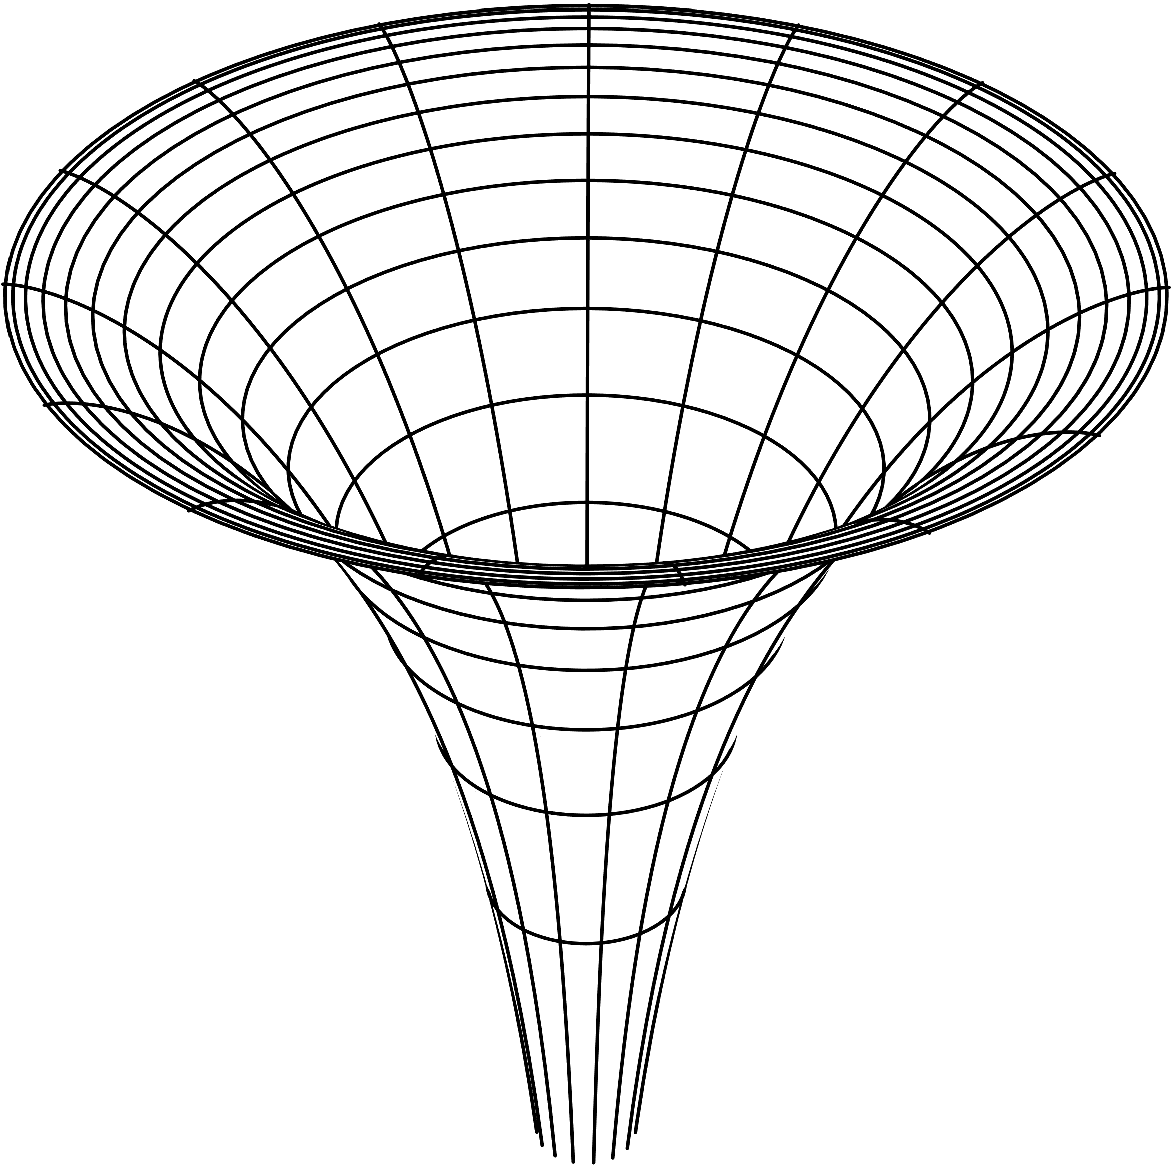
\includegraphics[width=6cm]{./img/Pseudosphere.pdf}
	\caption{Псевдосфера}
\end{figure}

\pagebreak

\begin{solution}
	\begin{enumerate}[nolistsep, label=(\arabic*)]
		\item Напрямую вычисляем коэффициенты\footnotemark:
			\begin{gather*}
				\vec{r}_u = \br{a\cos u\cos v,\,a\cos u\sin v,\,a\ctg u\cos u},\quad \vec{r}_v = (-a\sin u\sin v,\,a\sin u\cos v, 0),\\
				g_{11} = \langle\vec{r}_u, \vec{r}_u\rangle = a^2\cos^2u\big(\underbrace{(\cos^2v + \sin^2v)}_1 + \ctg^2u\big) = a^2\cos^2u\underbrace{(1 + \ctg^2u)}_{1 / \sin^2u} = a^2\ctg^2u,\\
				g_{12} = \langle\vec{r}_v, \vec{r}_v\rangle = -\cancel{\frac{a^2}{4}\sin2u\sin2v} + \cancel{\frac{a^2}{4}\sin2u\sin2v} = 0,\\
				g_{22} = \langle\vec{r}_v, \vec{r}_v\rangle = a^2\sin^2u\underbrace{(\sin^2v + \sin^2v)}_1 = a^2\sin^2u.
			\end{gather*}%
			\footnotetext{Выкладка: $\ds\br{\ln\tg\frac{u}{2}}^\prime = \frac{1}{\tg\frac{u}{2}} \cdot \frac{1}{\cos^2\frac{u}{2}} \cdot \frac{1}{2} = \frac{1}{2\sin\frac{u}{2}\cos\frac{u}{2}} = \frac{1}{\sin u}$.}%
			Пишем первую квадратичную форму:
			\[
				ds^2 = a^2\ctg^2u\,du^2 + a^2\sin^2u\,dv^2.
			\]
		\item Считаем частные производные, пользуясь формулами Френе:
			\[
				\vec{r}_t = \vec{v} + \lambda\dot{\vec{n}} = \vec{v} + \lambda(-k\vec{v} + \varkappa\vec{b}) = (1 - k\lambda)\vec{v} + \varkappa\lambda\vec{b},\quad \vec{r}_\lambda = \vec{n}.
			\]
			Вычисляем коэффициенты первой квадратичной формы:
			\begin{gather*}
				g_{11} = \langle\vec{r}_t, \vec{r}_t\rangle = (1 - k\lambda)^2 + \varkappa^2\lambda^2,\\
				g_{12} = \langle\vec{r}_t, \vec{r}_\lambda\rangle = 0,\\
				g_{22} = \langle\vec{r}_\lambda, \vec{r}_\lambda\rangle = 1.
			\end{gather*}
			Итак, выписываем первую квадратичную форму:
			\[
				ds^2 = \big((1 - k\lambda)^2 + \varkappa^2\lambda^2\big)dt^2 + d\lambda^2.
			\]
	\end{enumerate}
\end{solution}

\begin{problem}
	Найти угол между пересекающимися кривыми $u + v = 0$ и $u - v = 0$ на \textit{геликоиде} --- поверхности вида
	\[
		\vec{r}(u, v) = (u\sin v, u\cos v, av),
	\]
	где $u, v \in \R$, $a > 0$.
\end{problem}

\begin{figure}[H]
	\centering
	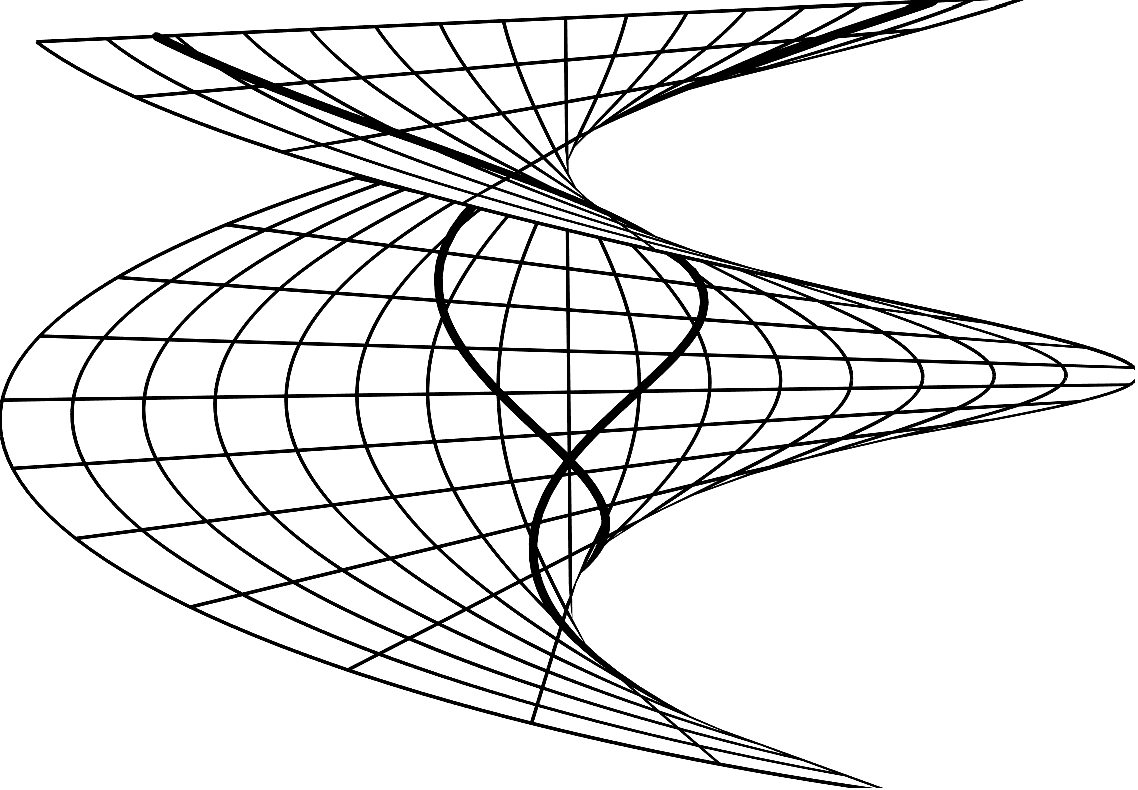
\includegraphics[width=6cm]{./img/HelicoidCurves.pdf}
	\caption{Две линии на геликоиде}
\end{figure}

\begin{solution}
	Посчитаем первую квадратичную форму нашей поверхности.
	\begin{gather*}
		\vec{r}_u = (\sin v, \cos v, 0),\quad \vec{r}_v = (u\cos v, -u\sin v, a),\\
		g_{11} = \langle\vec{r}_u, \vec{r}_u\rangle = {\underbrace{\sin^2v + \cos^2v}_{1}} = 1,\quad g_{12} = \langle\vec{r}_u, \vec{r}_v\rangle = 0,\\
		g_{22} = \langle\vec{r}_v, \vec{r}_v\rangle = u^2{\underbrace{(\sin^2v + \cos^2v)}_{1}} + a^2 = u^2 + a^2,\\
		\G(u, v) =
		\begin{pmatrix}
			1 & 0\\
			0 & u^2 + a^2
		\end{pmatrix}.
	\end{gather*}

	Данные кривые легко запараметризовать: $(t, -t)$ и $(t, t)$. Они пересекаются в точке $(0, 0)$. Их вектора скорости в этой точке есть $\vec{v}_1 = (1, -1)$ и $\vec{v}_2 = (1, 1)$ соответственно. Угол между кривыми находим по формуле
	\[
		\cos\angle(\vec{v}_1, \vec{v}_2) = \frac{\langle\vec{v}_1, \vec{v}_2\rangle|_{\G(0, 0)}}{\sqrt{\langle\vec{v}_1, \vec{v}_1\rangle|_{\G(0, 0)}}\sqrt{\langle\vec{v}_2, \vec{v}_2\rangle|_{\G(0, 0)}}} = \frac{1 - a^2}{1 + a^2}.
	\]
	Отсюда $\ds\angle(\vec{v}_1, \vec{v}_2) = \arccos\frac{1 - a^2}{1 + a^2}$.
\end{solution}

\begin{definition}
	\textit{Площадью} области $U$ на поверхности $\vec{r} = \vec{r}(u, v)$ называется величина
	\[
		\sigma(U) \vcentcolon = \iint\limits_{U}\sqrt{\deg\G}\,dudv.
	\]
	(Здесь область $U$ задана параметрически координатами $u$ и $v$.)
\end{definition}

Это определение (как и определение длины кривой) принимается как данность. Мотивировка такого определения в том, что $\sqrt{\det\G}$ --- это (ориентированная) площадь параллелограмма, натянутого на касательные вектора $\vec{r}_u$ и $\vec{r}_v$. Для простоты изложения в рамках этого курса мы не касаемся дифференциальных форм объёма, более подробно эта тема будет обсуждаться в курсе дифференциальной геометрии и топологии.

Площадь можно определить таким же образом не только на поверхности, но и в целом для римановой метрики в криволинейных координатах.

\begin{problem}
	В модели геометрии Лобачевского в верхней полуплоскости найти площадь треугольника, ограниченного кривыми
	\[
		x = 0,\quad (x - 1)^2 + y^2 = 4,\quad x^2 + y^2 = 9.
	\]
\end{problem}

\begin{solution}
	Метрика в модели геометрии Лобачевского в верхней полуплоскости имеет вид
	\[
		ds^2 = \frac{dx^2 + dy^2}{y^2},
	\]
	и $\sqrt{\det\G(x, y)} = 1 / y^2$. Следовательно, площадь нашего треугольника равна
	\[
		\sigma(U) = \iint\limits_{U}\frac{1}{y^2}\,dxdy,
	\]
	что после перехода к повторному интегралу даёт выражение
	\begin{multline*}
		\sigma(U) = \int\limits_0^3 dx\int\limits_{\sqrt{4 - (x - 1)^2}}^{\sqrt{9 - x^2}}\frac{1}{y^2}\,dy = \int\limits_0^3\br{\frac{1}{\sqrt{4 - (x - 1)^2}} - \frac{1}{\sqrt{9 - x^2}}}dx =\\ = \left.\br{\arcsin\frac{x - 1}{2} - \arcsin\frac{x}{3}}\right|_0^3 = 0 - \br{-\frac{\pi}{6}} = \frac{\pi}{6}.
	\end{multline*}

	\begin{figure}[H]
		\centering
		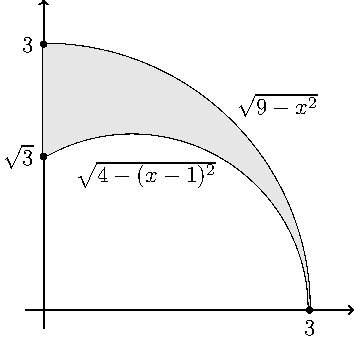
\includegraphics[width=6cm]{./img/CurveTriangle.pdf}
		\caption{Переход к повторному интегралу}
	\end{figure}
\end{solution}

\begin{example} В качестве доказательства пунктов $(2)$ и $(3)$ смотреть пример \ref{example:IFormOnSurfaces}.
	\begin{enumerate}[nolistsep, label=(\arabic*)]
		\item Если поверхность задана в параметрической форме $\vec{r} = \vec{r}(u, v)$ и $V$ --- такая область на плоскости $(u, v)$, что $\vec{r}(V) = U$, то
			\[
				\sigma(U) = \iint\limits_{V}\abs{\vec{r}_u \times \vec{r}_v}dudv.
			\]
		\item Если поверхность задана как график функции $z = f(x, y)$ и область $U$ проектируется на область $V$ на плоскости $(x, y)$, то
			\[
				\sigma(U) = \iint\limits_{V}\sqrt{1 + f_x^2 + f_y^2}\,dxdy.
			\]
		\item Если поверхность задана уравнением $F(x, y, z) = 0$, $F_z \ne 0$ в области $U$, которая проектируется на область $V$ на плоскости $(x, y)$. Тогда
			\[
				\sigma(U) = \iint\limits_{V}\frac{\abs{\grad F}}{\abs{F_z}}\,dxdy.
			\]
	\end{enumerate}
\end{example}

\begin{problem}
	Найти площадь тора
	\[
		\begin{cases}
			x = (R + r\cos\psi)\cos\varphi,\\
			y = (R + r\cos\psi)\sin\varphi,\\
			z = r\sin\psi,
		\end{cases}
	\]
	где $r < R$, $0 \leqslant \varphi, \psi < 2\pi$.
\end{problem}

\begin{figure}[H]
	\centering
	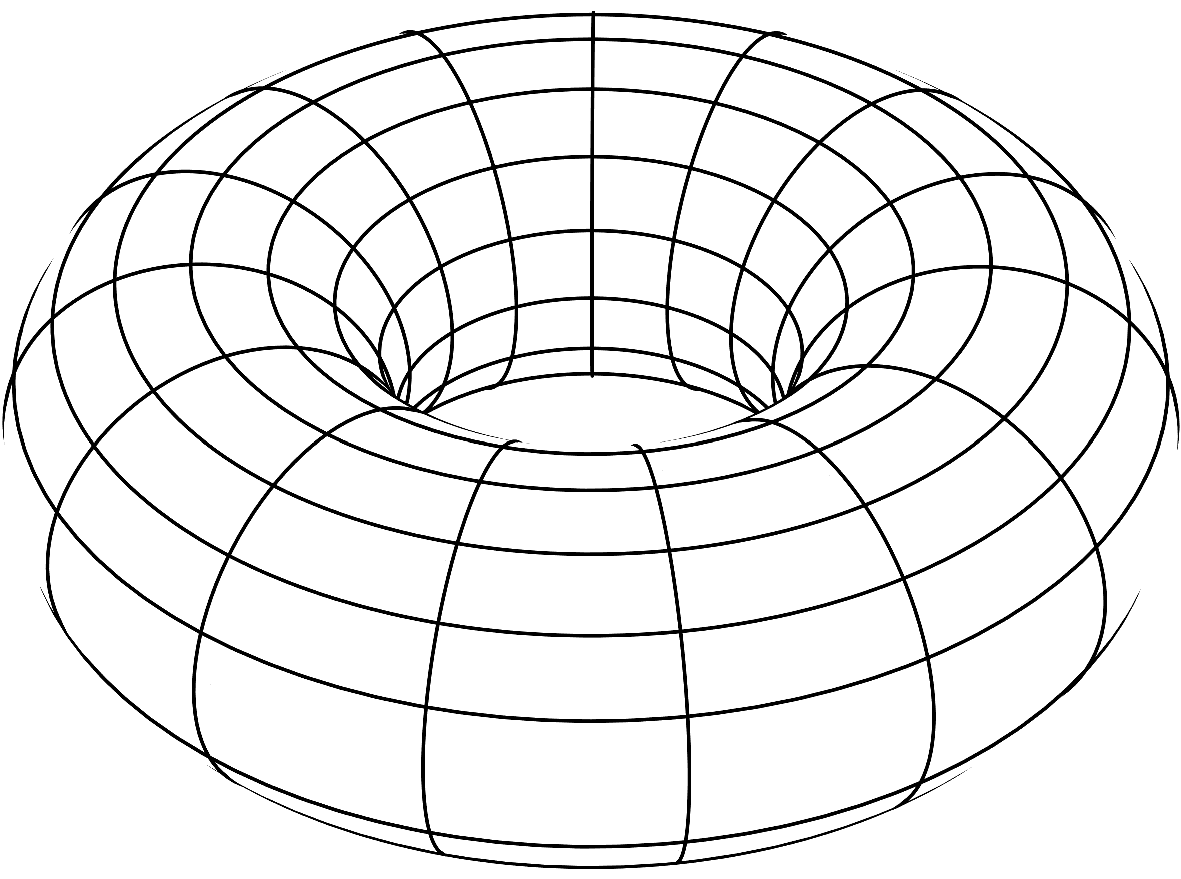
\includegraphics[width=6cm]{./img/Torus.pdf}
	\caption{Тор}
\end{figure}

\begin{solution}
	Находим частные производные радиус-вектора:
	\begin{gather*}
		\vec{r}_\varphi = (R + r\cos\psi)\big({-\sin\varphi}, \cos\varphi, 0\big),\\
		\vec{r}_\psi = r\big({-\cos\varphi\sin\psi}, -\sin\varphi\sin\psi, \cos\psi\big),
	\end{gather*}
	затем риманову метрику на торе:
	\[
		\G =
		\begin{pmatrix}
			(R + r\cos\psi)^2 & 0\\
			0 & r^2
		\end{pmatrix}.
	\]
	Считаем искомую площадь:
	\begin{multline*}
		\sigma = \iint\limits_{\varphi, \psi}\sqrt{\det\G}\,d\varphi d\psi = \int\limits_0^{2\pi}d\varphi\int\limits_0^{2\pi}(R + r\cos\psi)r\,d\psi =\\ = 2\pi r\int\limits_0^{2\pi}(R + r\cos\psi)\,d\psi = 2\pi r \cdot 2\pi R = 4\pi^2 Rr.
	\end{multline*}
\end{solution}

Из существования натурального параметра на кривой следует, что каждый участок кривой можно отобразить в прямую с сохранением расстояний между точками. Двумерные поверхности в трехмерном евклидовом пространстве уже обладают внутренней геометрией. В общем случае никакая окрестность точки поверхности не может быть отображена на область в евклидовой плоскости с сохранением расстояний.

\begin{definition}
	Говорят, что поверхности $\M$ и $\mathcal{N}$ \textit{изометричны}, если между ними существует диффеоморфизм $\vec{\varphi}\colon \M \to \mathcal{N}$, который сохраняет длины всех кривых. Сам дифферморфизм $\vec{\varphi}$ называется при этом \textit{изометрией}.
\end{definition}

\noindent
Гладкое отображение поверхностей
\[
	\vec{f}\colon (u^1, u^2) \mapsto (\widetilde{u}^1(u^1, u^2), \widetilde{u}^2(u^1, u^2)),
\]
записанное в локальных координатах, сохраняет длины всех кривых, если и только если
\begin{equation} \label{eq:Isometry}
	\widetilde{g}_{ij}\big|_{\vec{f}(u^1, u^2)}\,d\widetilde{u}^id\widetilde{u}^j = g_{kl}\big|_{(u^1, u^2)}\,du^kdu^l,
\end{equation}
где $g_{kl}\,du^kdu^l$ и $\widetilde{g}_{ij}\,d\widetilde{u}^id\widetilde{u}^j$ --- первые квадратичные формы поверхностей. Идейно тут всё понятно --- это условие и означает, что на поверхностях <<одинаково измеряются расстояния>>. Распишем строго: пусть $\vec{r}(t) = (u^1(t), u^2(t))$ --- кривая и $\widetilde{\vec{r}}(t)$ --- её образ, $a \leqslant t \leqslant b$,
\[
	\int\limits_a^b\sqrt{g_{kl}(\vec{r}(t))\,\dot{u}^k\dot{u}^l}\,dt = \int\limits_a^b\sqrt{\widetilde{g}_{ij}(\widetilde{\vec{r}}(t))\,\dot{\widetilde{u}}{}^i\dot{\widetilde{u}}{}^j}\,dt.
\]

При изометрии это равенство выполняется для любой кривой $\vec{r}(t)$, что равносильно соотношению \eqref{eq:Isometry}.

\begin{problem}
	Доказать, что \textit{геликоид}:
	\[
		\vec{r}(u, v) = (u\sin v, u\cos v, v),
	\]
	где $u, v \in \R$, локально изометричен \textit{катеноиду}:
	\[
		\widetilde{\vec{r}}(u, v) = (\ch u\cos v, \ch u\sin v, u),
	\]
	где $u \in \R$, $0 \leqslant v < 2\pi$.
\end{problem}

\begin{figure}[H]
	\centering
	\begin{minipage}{.4\textwidth}
		\centering
		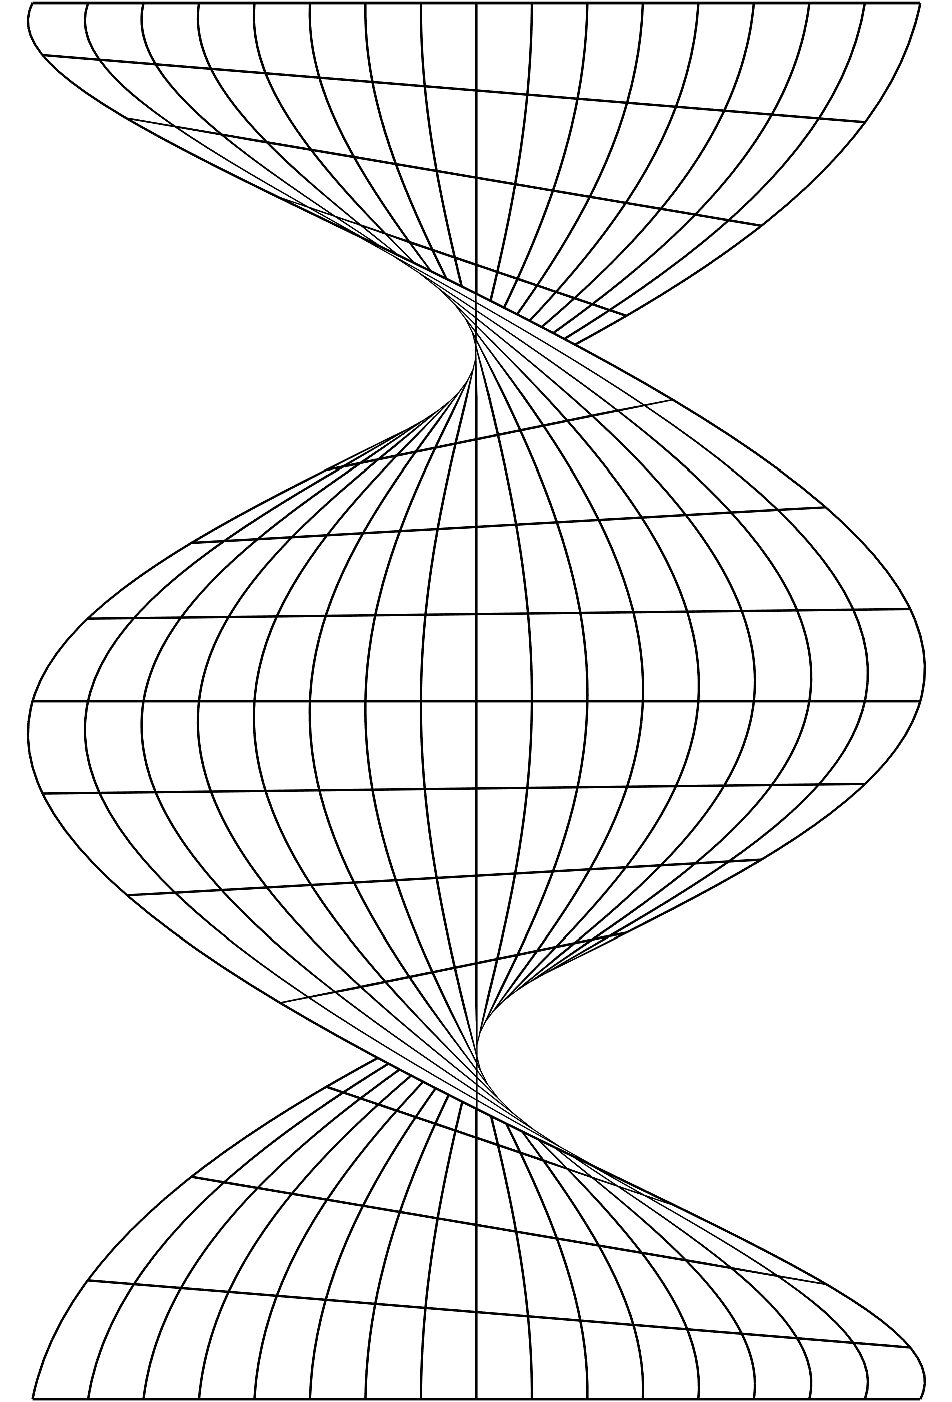
\includegraphics[width=5cm]{./img/Helicoid.pdf}
	\end{minipage}
	\begin{minipage}{.4\textwidth}
		\centering
		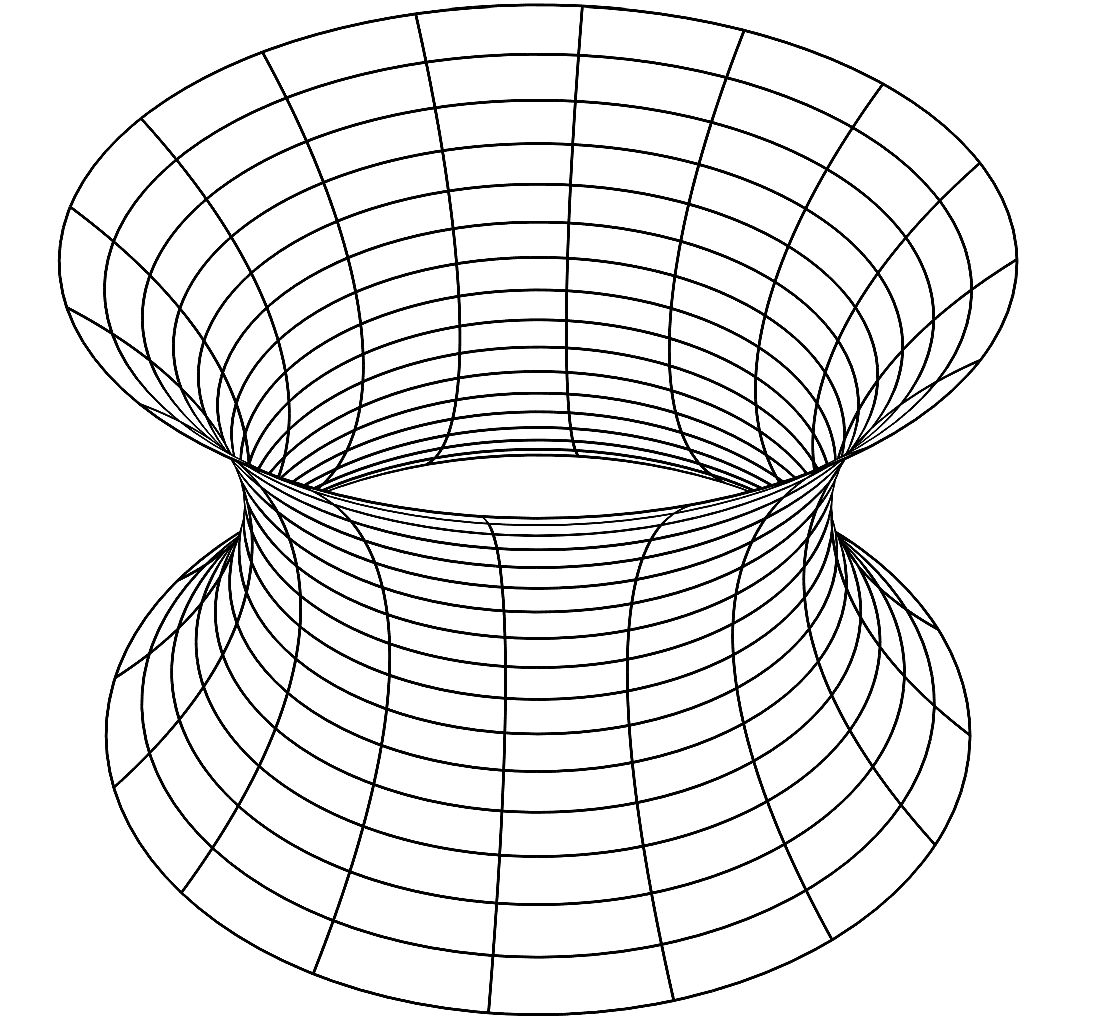
\includegraphics[width=5cm]{./img/Catenoid.pdf}
	\end{minipage}
	\vspace{.3cm}

	\begin{minipage}{.4\textwidth}
		\centering
		Геликоид
	\end{minipage}
	\begin{minipage}{.4\textwidth}
		\centering
		Катеноид
	\end{minipage}
	
	\caption[format=empty]{}
	\label{fig:HelicoidCatenoid}
\end{figure}

\begin{solution}
	Нужно посчитать первые квадратичные формы обеих поверхностей и найти дифферморфизм, сохраняющий длины кривых. Для геликоида:
	\begin{gather} \label{eq:HelicoidI}
		\vec{r}_u = (\sin v, \cos v, 0),\quad \vec{r}_v = (u\cos v, -u\sin v, 1),\nonumber\\
		g_{11} = \langle\vec{r}_u, \vec{r}_u\rangle = {\underbrace{\sin^2v + \cos^2v}_{1}} = 1,\quad g_{12} = \langle\vec{r}_u, \vec{r}_v\rangle = 0,\nonumber\\
		g_{22} = \langle\vec{r}_v, \vec{r}_v\rangle = u^2{\underbrace{(\sin^2v + \cos^2v)}_{1}} + 1 = u^2 + 1,\nonumber\\
		ds^2 = du^2 + (u^2 + 1)\,dv^2.
	\end{gather}
	Для катеноида:
	\begin{gather}
		\widetilde{\vec{r}}_{\widetilde{u}} = (\sh \widetilde{u}\cos \widetilde{v}, \sh \widetilde{u}\sin \widetilde{v}, 1),\quad \widetilde{\vec{r}}_{\widetilde{v}} = (-\ch \widetilde{u}\sin \widetilde{v}, \ch \widetilde{u}\cos \widetilde{v}, 0),\nonumber\\
		\widetilde{g}_{11} = \langle\widetilde{\vec{r}}_{\widetilde{u}}, \widetilde{\vec{r}}_{\widetilde{u}}\rangle = \sh^2\widetilde{u}\,{\underbrace{(\cos^2\widetilde{v} + \sin^2\widetilde{v})}_{1}} + 1 = \sh^2\widetilde{u} + 1 = \ch^2\widetilde{u},\nonumber\\
		\widetilde{g}_{12} = \langle\widetilde{\vec{r}}_{\widetilde{u}}, \widetilde{\vec{r}}_{\widetilde{v}}\rangle = 0,\quad
		\widetilde{g}_{22} = \langle\widetilde{\vec{r}}_{\widetilde{v}}, \widetilde{\vec{r}}_{\widetilde{v}}\rangle = \ch^2\widetilde{u}\,{\underbrace{(\sin^2\widetilde{v} + \cos^2\widetilde{v})}_{1}} = \ch^2\widetilde{u},\nonumber\\
		d\widetilde{s}^2 = \ch^2\widetilde{u}\,d\widetilde{u}^2 + \ch^2\widetilde{u}\,d\widetilde{v}^2. \label{eq:CatenoidI}
	\end{gather}

	Теперь нужно подобрать диффеоморфизм $u = u(\widetilde{u})$, $v = v(\widetilde{v})$ такой, что форма \eqref{eq:HelicoidI} перейдёт в \eqref{eq:CatenoidI}. Никаких общих методов для этого нет, только смекалка. Здесь, например, подойдёт отображение $u = \sh\widetilde{u}$, $v = \widetilde{v}$. Действительно,
	\[
		du^2 = (d\sh\widetilde{u})^2 = \ch^2\widetilde{u}^2\,d\widetilde{u}^2,\quad(\sh^2\widetilde{u} + 1)\,d\widetilde{v}^2 = \ch^2\widetilde{u}\,d\widetilde{v}^2.
	\]
\end{solution}

\begin{problem}
	Доказать, что деформация гиперболического параболоида, определяемая следующими формулами, сохраняет площадь:
	\[
		\begin{cases}
			x = u,\\
			y = v,\\
			\ds z = \frac{1}{2}(u^2 - v^2)
		\end{cases}
		\mapsto
		\begin{cases}
			x = u,\\
			y = v,\\
			\ds z = \frac{\sin t}{2}(u^2 - v^2) + uv\cos t.
		\end{cases}
	\]
\end{problem}

\begin{solution} % TODO: Решить!
	Появится позже.
\end{solution}

% TODO: Написать про конформные отображения + условия Коши-Римана!

\subsection{Кривизна поверхности}

Сначала мы дадим <<дурацкое>> определение, а затем предоставим к нему исчерпывающую мотивацию. Рассмотрим поверхность, заданную параметрически: $\vec{r} = \vec{r}(u, v)$. Зададим к ней нормаль $\vec{n}$ в каждой точке:
\[
	\vec{n} \vcentcolon = \frac{\vec{r}_u \times \vec{r}_v}{\abs{\vec{r}_u \times \vec{r}_v}}.
\]

\begin{definition}
	\textit{Вторую квадратичную форму} определим как выражение
	\[
		L\,du^2 + 2M\,dudv + N\,dv^2,
	\]
	где
	\[
		L \vcentcolon = \langle\vec{r}_{uu}, \vec{n}\rangle,\quad M \vcentcolon = \langle\vec{r}_{uv}, \vec{n}\rangle,\quad N \vcentcolon = \langle\vec{r}_{vv}, \vec{n}\rangle.
	\]
	Полагая $u^1 = u$, $u^2 = v$, будем также записывать её в виде
	\[
		b_{ij}\,du^idu^j,
	\]
	где
	\[
		\B = \begin{pmatrix}
			b_{11} & b_{12}\\
			b_{12} & b_{22}
		\end{pmatrix} \vcentcolon =
		\begin{pmatrix}
			L & M\\
			M & N
		\end{pmatrix}.
	\]
\end{definition}

Для второй квадратичной формы, как и для первой, нужно доказать корректность определения --- то есть независимость от системы координат, в которой она записывается. Мы не будем утруждать себя лобовым доказательством тензорного закона, а увидим, что вторая квадратичная форма имеет геометрический смысл, инвариантный относительно выбора системы координат.

Рассмотрим кривую $\vec{\rho} = \vec{\rho}(u(t), v(t))$ на нашей поверхности, параметризованную в локальных координатах в окрестности точки $\vec{r}(u_0, v_0) \ni \Im\vec{\rho}$. Нормаль к поверхности в этой точке обозначим через $\vec{n}$. Тогда имеем (здесь через точку обозначена производная по $t$)
\begin{gather*}
	\ddot{\vec{\rho}} = \vec{\rho}_{uu}\dot{u}^2 + 2\vec{\rho}_{uv}\dot{u}\dot{v} + \vec{\rho}_{vv}\dot{v}^2 + \vec{\rho}_u\ddot{u} + \vec{\rho}_v\ddot{v},\\
	\langle\ddot{\vec{\rho}}, \vec{n}\rangle = L\dot{u}^2 + 2M\dot{u}\dot{v} + M\dot{v}^2,
\end{gather*}
так как $\vec{\rho}_u \perp \vec{n}$ и $\vec{\rho}_v \perp \vec{n}$. Получается, что значение второй квадратичной формы на векторе скорости кривой $\vec{\rho}$ (который, конечно же, является касательным вектором к поверхности) есть длина проекции вектора ускорения этой кривой на нормаль к поверхности.

Теперь имеем полное право называть определённое выше выражение квадратичной формой, обозначим её через $\II$. Попутно мы доказали следующее предложение.

\begin{proposition} \label{proposition:GeomII}
	Если $\vec{\rho} = \vec{\rho}(u(t), v(t))$ --- гладкая кривая на поверхности, то
	\[
		\langle\ddot{\vec{\rho}}, \vec{n}\rangle = \II(\dot{\vec{\rho}}).
	\]
\end{proposition}

\noindent%
Позже мы вернёмся к этому сюжету, но пока вынуждены отступить от него.

\subsection{Главные кривизны и нормальные сечения}

Подытожим наши рассуждения. В касательном пространстве к каждой точке поверхности определены две квадратичные формы --- $\I$ и $\II$, --- при этом форма $\I$ положительно определена. Из курса линейной алгебры известно, что тогда эти квадратичные формы можно привести к главным осям, то есть выбрать базис (в касательном пространстве), в котором матрица формы $\I$ будет единичной, а матрица формы $\II$ --- диагональной.

% TODO: убрать "скоро там всё появится", когда допишешь в теорминимум

Кратно напомним, как это делать (подробные объяснения и теоретические обоснования смотреть в \href{https://github.com/pshenikita/Linal-Teormin}{теорминимуме}, скоро там всё появится). Сначала нужно найти собственные значение пары квадратичных форм, то есть решить уравнение
\begin{equation} \label{eq:MainAxes}
	\det(\B - \lambda\G) = 0
\end{equation}
относительно $\lambda$, где $\G$ и $\B$ --- матрицы первой и второй квадратичной формы в каком-то базисе касательного пространства. Сразу отметим, что само уравнение \eqref{eq:MainAxes} инвариантно относительно замены координат и определяется самой поверхностью. Поэтому его коэффициенты в развёрнутом и приведённом виде
\[
	\lambda^2 -H\lambda + K = 0
\]
имеет смысл как-то обозначить.

\begin{definition}
	Коэффициент $H$ называется \textit{средней кривизной} поверхности в данной точке\footnotemark, а коэффициент $K$ --- \textit{гауссовой кривизной}. Корни $\lambda_1$ и $\lambda_2$ уравнения \eqref{eq:MainAxes} называются \textit{главными кривизнами}. (По теореме Виета имеем $H = \lambda_1 + \lambda_2$, $K = \lambda_1\lambda_2$.)
\end{definition}

\footnotetext{<<Данная точка>> здесь --- это та, в касательном пространстве к которой мы сейчас находимся.}

Обычно среднюю кривизну определяют как среднее арифметическое главных кривизн, но такое определение влечёт лишь к небольшому усложнению формул за счёт возникновения множителя $1 / 2$. Все эти кривизны имеют для нас \underline{фундаментальное} значение. Их очень глубокий геометрический смысл будет ясен позднее.

Если $\lambda_1 \ne \lambda_2$, то главные направления $\vec{\xi}_1$ и $\vec{\xi}_2$ ортогональны и находятся из уравнений
\[
	(\B - \lambda_iG)\vec{\xi}_i = \vec{0},
\]
где $i = 1, 2$.

А если $\lambda_1 = \lambda_2$, то первая и вторая квадратичные формы пропорциональны, и любые векторы подойдут как главные направления. Такие точки называются \textit{омбилическими}.

Лобовым раскрытием скобок можем получить явные формулы для гауссовой и средней кривизн через коэффициенты первой и второй квадратичных форм:
\[
	K = \frac{g_{11}g_{22} - g_{12}^2}{b_{11}b_{22} - b_{12}^2} = \frac{\det\G}{\det\B},\qquad H = \frac{g_{11}b_{22} + g_{22}b_{11} - 2g_{12}b_{12}}{g_{11}g_{22} - g_{12}^2} = \tr(\G^{-1}\B).
\]

\begin{example}
	Пусть поверхность задана как график функции $z = f(x, y)$. Тогда
	\begin{gather*}
		\vec{r}_x = (1, 0, f_x),\quad \vec{r}_{y} = (0, 1, f_y),\quad \vec{r}_x \times \vec{r}_y = (-f_x, -f_y, 1),\\
		\vec{r}_{xx} = (0, 0, f_{xx}),\quad \vec{r}_{xy} = (0, 0, f_{xy}),\quad \vec{r}_{yy} = (0, 0, f_{yy}),\\
		\vec{n} = \frac{\vec{r}_x \times \vec{r}_y}{\abs{\vec{r}_x \times \vec{r}_y}} = \frac{(-f_x, -f_y, 1)}{\sqrt{1 + f_x^2 + f_y^2}},\\
		b_{11} = \frac{f_{xx}}{\sqrt{1 + f_x^2 + f_y^2}},\quad b_{12} = \frac{f_{xy}}{\sqrt{1 + f_x^2 + f_y^2}},\quad b_{22} = \frac{f_{yy}}{\sqrt{1 + f_x^2 + f_y^2}}.
	\end{gather*}
	Отсюда, гауссова кривизна поверхности, заданной в виде графика, равна
	\[
		K = \frac{\det\G}{\det\B} = \frac{(1 + f_x^2)(1 + f_y^2) - f_x^2f_y^2}{(1 + f_x^2 + f_y^2)^2} = \frac{f_{xx}f_{yy} - f_{xy}^2}{(1 + f_x^2 + f_y^2)^2}.
	\]
\end{example}

\begin{problem}
	Найти главные направления, гауссову и среднюю кривизны у псевдосферы
	\[
		x = a\sin u\cos v,\quad y = a\sin u\sin v,\quad z = a\br{\ln\tg\frac{u}{2} + \cos u},
	\]
	где $0 < u < \pi / 2$, $0 \leqslant v < 2\pi$, $a \ne 0$.
\end{problem}

\begin{solution}
	Первую квадратичную форму у псевдосферы мы уже считали в задаче \ref{problem:FindG}, получили
	\[
		\G =
		\begin{pmatrix}
			a^2\ctg^2u & 0\\
			0 & a^2\sin^2u
		\end{pmatrix}.
	\]

	Посчитаем вторую квадратичную форму. Для этого нам нужно считать вторые производные от параметризации $\vec{r}$ нашей поверхности. Первые, опять же, мы уже считали:
	\[
		\vec{r}_u = (a\cos u\cos v, a\cos u\sin v, a\ctg u\cos u),\quad\vec{r}_v = (-a\sin u\sin v, a\sin u\cos v, 0).
	\]
	Считаем вторые:
	\begin{gather*}
		\vec{r}_{uu} = \big({-a\sin u\cos v}, -a\sin u\sin v, -a\cos u(2 + \ctg^2u)\big),\\
		\vec{r}_{uv} = (-a\cos u\sin v, a\cos u\cos v, 0),\\
		\vec{r}_{vv} = (-a\sin u\cos v, -a\sin u\sin v, 0).
	\end{gather*}
	Находим вектор нормали:
	\begin{multline*}
		\vec{r}_u \times \vec{r}_v = \det
		\begin{pmatrix}
			\vec{e}_1 & \vec{e}_2 & \vec{e}_3\\
			a\cos u\cos v & a\cos u\sin v & a\ctg u\cos u\\
			-a\sin u\sin v & a\sin u\cos v & 0
		\end{pmatrix} =\\ = a^2 \br{{-\cos^2u\cos v}, -\cos^2u\sin v, \frac{1}{2}\sin 2u}.
	\end{multline*}
	\begin{multline*}
		\abs{\vec{r}_u \times \vec{r}_v}^2 = a^4{\cos^4u\underbrace{(\cos^2v + \sin^2v)}_{1}} + \frac{1}{4}a^4\sin^22u =\\ = a^4\big(\cos^4u + \cos^2u(1 - \cos^2u)\big) = a^4\cos^2u,
	\end{multline*}
	\begin{gather*}
		\vec{n} = \frac{\vec{r}_u \times \vec{r}_v}{\abs{\vec{r}_u \times \vec{r}_v}} = (-\cos u\cos v, -\cos u\sin v, \sin u).
	\end{gather*}
	Теперь можем найти коэффициенты второй квадратичной формы:
	\begin{multline*}
		b_{11} = \langle\vec{r}_{uu}, \vec{n}\rangle = {a\cos u\sin u\underbrace{(\cos^2 v + \sin ^2 v)}_{1}} - a\sin u\cos u(2 + \ctg^2u) =\\ = {-a\sin u\cos u\underbrace{(1 + \ctg^2 u)}_{1 / \sin^2u}} = -a\ctg u,
	\end{multline*}
	\begin{gather*}
		b_{12} = \langle\vec{r}_{uv}, \vec{n}\rangle = 0,\\
		b_{22} = \langle\vec{r}_{vv}, \vec{n}\rangle = {a\cos u\sin u\underbrace{(\cos^2 v + \sin ^2 v)}_{1}} = \frac{a}{2}\sin 2u.
	\end{gather*}
	Можем выписать матрицу второй квадратичной формы:
	\[
		\B =
		\begin{pmatrix}
			-a\ctg u & 0\\
			0 & \frac{a}{2}\sin 2u
		\end{pmatrix}.
	\]
	Находим главные кривизны:
	\begin{gather*}
		\det(\B - \lambda\G) = 0,\\
		\det
		\begin{pmatrix}
			-\ctg u - a\lambda \ctg^2u & 0\\
			0 & \frac{1}{2}\sin 2u - a\lambda \sin^2u
		\end{pmatrix} = 0,\\
		a^2\cos^2u \cdot \lambda^2 + a\br{{-\frac{\cos^3u}{\sin u}} + \cos u\sin u} \cdot \lambda -\cos^2 u = 0,\ \ \big|\ {:}\,a^2\cos^2u\\
		\lambda^2 - \frac{\ctg u - \tg u}{a}\lambda - \frac{1}{a^2} = 0.
	\end{gather*}

	Отсюда, $\lambda_1 = -a^{-1}\tg u$, $\lambda_2 = a^{-1}\ctg u$ и $H = a^{-1}(\ctg u - \tg u)$, $K \equiv -a^{-2}$. Наконец, можем найти главные направления.
	\begin{gather*}
		(\B - \lambda_1\G)\vec{\xi}_1 = \vec{0},\\
		\begin{pmatrix}
			0 & 0\\
			0 & \tg u
		\end{pmatrix}\vec{\xi}_1 = \vec{0}.
	\end{gather*}
	В качестве решения подойдёт, например, вектор $\vec{\xi}_1 = (1, 0)$. Ищем второй вектор:
	\begin{gather*}
		(\B - \lambda_2\G)\vec{\xi}_2 = \vec{0},\\
		\begin{pmatrix}
			-\frac{\cos u}{\sin^3 u} & 0\\
			0 & 0
		\end{pmatrix}\vec{\xi}_2 = \vec{0}.
	\end{gather*}

	Здесь подойдёт вектор $\vec{\xi}_2 = (0, 1)$. Итак, мы нашли главные направления в базисе $(\vec{r}_u, \vec{r}_v)$ касательного пространства. Можно записать их и в базисе $\R^3$, в котором находится наша поверхность. Для этого пишем $\vec{\xi}_i = \xi_i^1\vec{r}_u + \xi_i^2\vec{r}_v$. В данном случае всё очевидно --- $\vec{\xi}_1 = \vec{r}_u$, $\vec{\xi}_2 = \vec{r}_v$. Нам повезло, и векторы изначального базиса $(\vec{r}_u, \vec{r}_v)$ оказались главными направлениями. Так происходит редко, в общем случае мы найдём подходящие векторы, нормируем их и запишем в трёхмерных координатах.
\end{solution}

С каждой неомбилической точкой гладкой поверхности можно связать ортонормированный базис $(\vec{\xi}_1, \vec{\xi}_2, \vec{n})$ из главных направлений и вектора единичной нормали. Вблизи этой точки можно задать нашу функцию как график $z = f(x, y)$, к такому заданию поверхностей мы уже обращались в примере \ref{example:IFormOnSurfaces}. С одной стороны, первая квадратичная форма имеет вид
\[
	\begin{pmatrix}
		1 + f_x^2 & f_xf_y\\
		f_xf_y & 1 + f_y^2
	\end{pmatrix}.
\]

Но с другой стороны, в базисе из главных направлений матрица первой квадратичной формы в рассматриваемой точке единичная, отсюда находим $f_x = f_y = 0$. В выбранном базисе имеем $\vec{n} = (0, 0, 1)$, поэтому легко находим и коэффициенты второй квадратичной формы:
\[
	\begin{pmatrix}
		f_{xx} & f_{xy}\\
		f_{xy} & f_{yy}
	\end{pmatrix},
\]
при этом в выбранном базисе эта форма диагональна, то есть $f_{xy} = 0$. Таким образом, имеем следующие матрицы квадратичных форм:
\[
	\G =
	\begin{pmatrix}
		1 & 0\\
		0 & 1
	\end{pmatrix},\qquad
	\B =
	\begin{pmatrix}
		f_{xx} & 0\\
		0 & f_{yy}
	\end{pmatrix}.
\]

Сразу видим главные кривизны: $\lambda_1 = f_{xx}$, $\lambda_2 = f_{yy}$. Можно написать разложение функции $z = f(x, y)$ в ряд Тейлора, которое в нашем случае выглядит так:
\begin{equation} \label{eq:TailorII}
	z = \frac{\lambda_1}{2}x^2 + \frac{\lambda_2}{2}y^2 + \o(x^2 + y^2).
\end{equation}

Отбросив $\o(x^2 + y^2)$, мы получим уравнение параболоида, который приближает нашу поверхность вблизи начала координат. Эта соприкасающайся поверхность второго порядка служит аналогом соприкасающейся окружности к кривой. В зависимости от вида этой приближающей поверхности, каждую неомбилическую точку поверхности можно отнести к одному из трёх типов.

\begin{definition}
	\begin{enumerate}[nolistsep, label=(\arabic*)]
		\item Если $\lambda_1$ и $\lambda_2$ оба ненулевые и одного знака ($K > 0$), то такая точка называется \textit{эллиптической} (в этом случае приближающая поверхность --- эллиптический параболоид).
		\item Если $\lambda_1$ и $\lambda_2$ разных знаков ($K < 0$), то такая точка называется \textit{гиперболической} (приближающая поверхность --- гиперболический параболоид).
		\item Если одно из $\lambda_1$ и $\lambda_2$ нулевое ($K = 0$), то такая точка называется \textit{параболической} (приближающая поверхность --- параболический цилиндр).
	\end{enumerate}
\end{definition}

\begin{figure}[H]
	\centering
	\begin{minipage}{.3\textwidth}
		\centering
		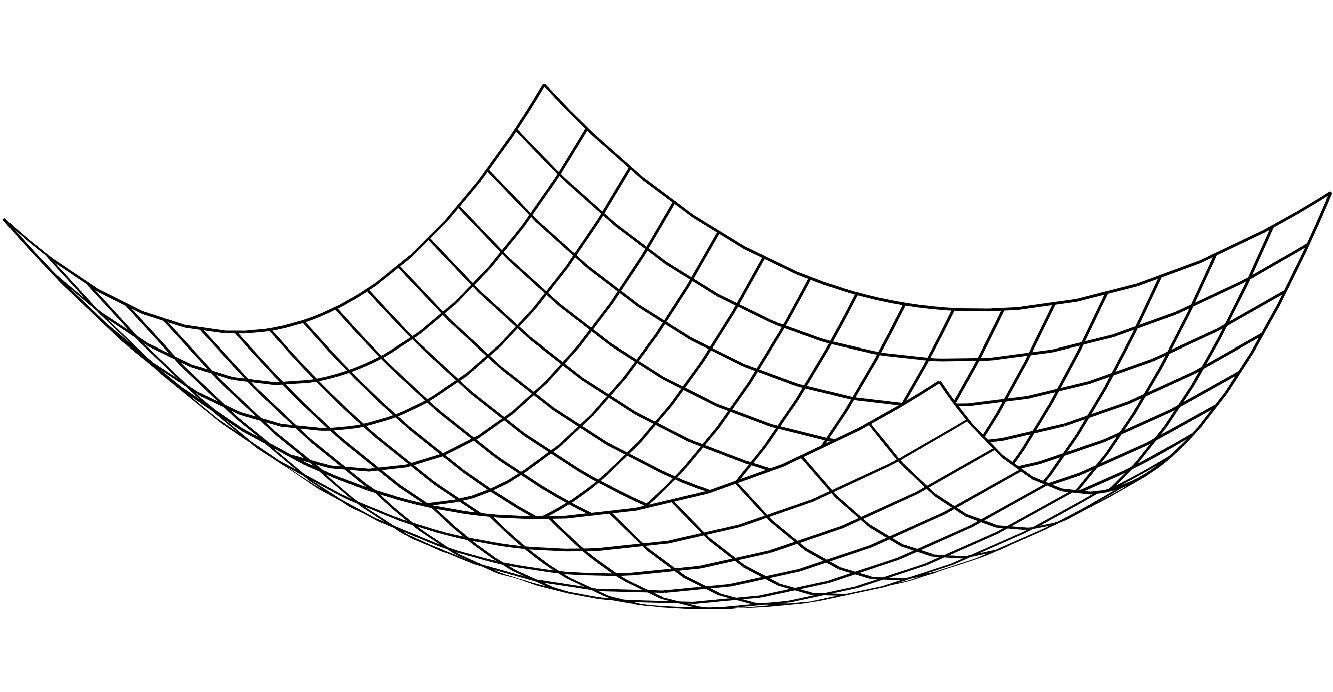
\includegraphics[height=2cm]{./img/Elliptic.pdf}

		$K > 0$
	\end{minipage}
	\begin{minipage}{.3\textwidth}
		\centering
		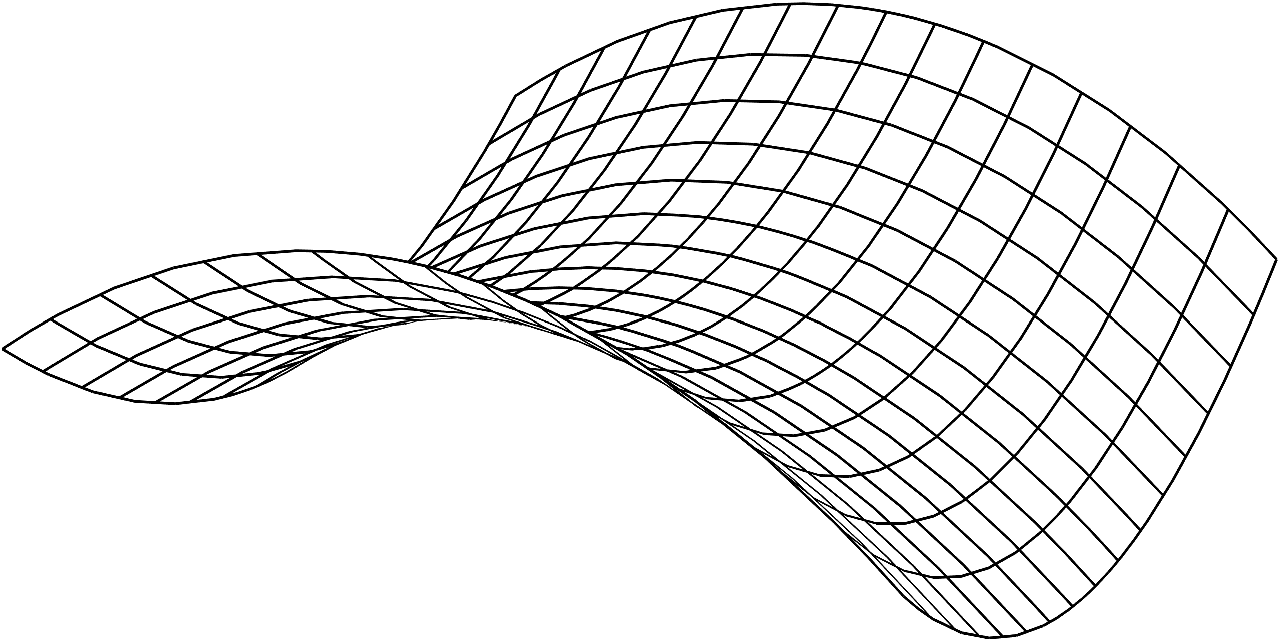
\includegraphics[height=2cm]{./img/Hyperbolic.pdf}

		$K < 0$
	\end{minipage}
	\begin{minipage}{.3\textwidth}
		\centering
		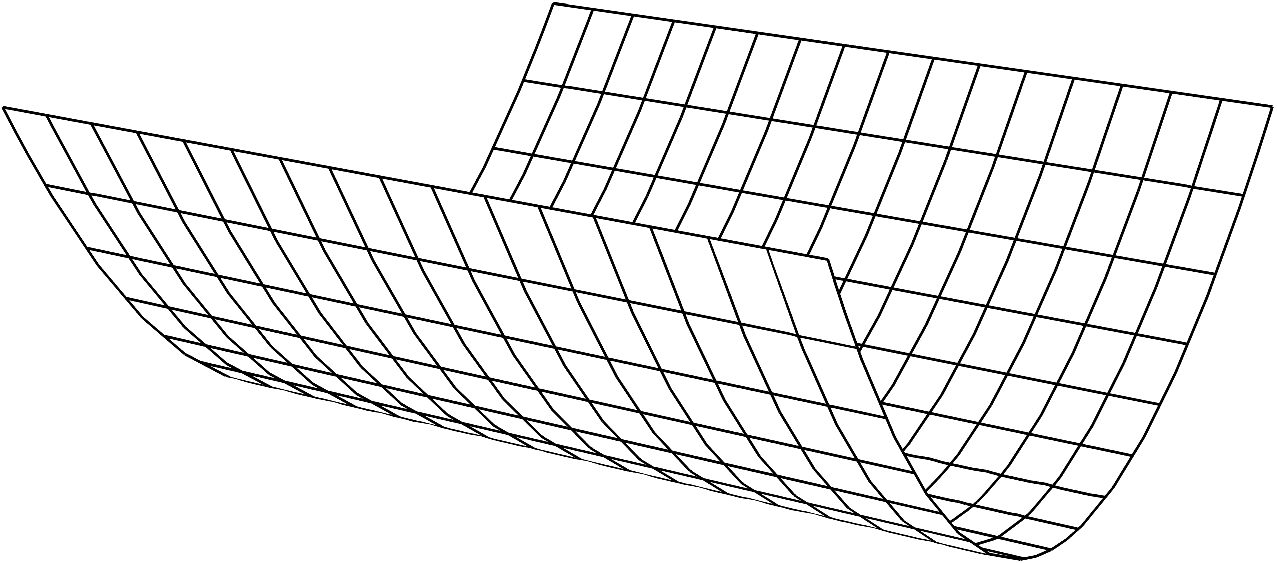
\includegraphics[height=2cm]{./img/Parabolic.pdf}

		$K = 0$
	\end{minipage}
	\caption{Вид соприкасающегося параболоида в зависимости от гауссовой кривизны}
\end{figure}

Далее мы опишем геометрический смысл главных кривизн и второй квадратичной формы, для этого мы будем рассматривать сечения поверхности плоскостями. 

\begin{definition}
	\textit{Нормальным сечением} поверхности $\M$ в некоторой точке $\vec{x} \in \M$ называется кривая в пересечении этой поверхности и плокости, порождённой каким-то касательным вектором $\vec{\xi} \in \T_{\vec{x}}\M$ и нормалью к поверхности в точке $\vec{x}$.
\end{definition}

Обратимся к предложению \ref{proposition:GeomII}. (Здесь также точками обозначены производые по $t$.) Обозначим через $\vec{n}_\rho$ вектор главной нормали кривой $\vec{\rho}$ в рассматриваемой точке, а через $\theta$ --- угол между ним и вектором нормали к поверхности, то есть $\theta = \angle(\vec{n}_\rho, \vec{n})$. Кривизна\footnotemark{} кривой $\vec{\rho}$ определяется из соотношения
\[
	\frac{d^2\vec{\rho}}{ds^2} = k_{\Or}\vec{n}_\rho,
\]
где $s$ --- натуральный параметр на кривой, то есть $ds$ --- метрика на нашей поверхности (вспомнить предложение \ref{proposition:LengthParameter}). Мы уже поняли, что
\[
	\left\langle\frac{d^2\vec{\rho}}{ds^2}, \vec{n}\right\rangle = b_{11}\br{\frac{du}{ds}}^2 + 2b_{12}\frac{du}{ds}\frac{dv}{ds} + b_{22}\br{\frac{dv}{ds}}^2 = \frac{b_{ij}\,du^idu^j}{ds^2},
\]
причём, из определения натурального параметра, $ds^2 = \abs{\dot{\vec{\rho}}}^2dt^2 = \I(\dot{\vec{\rho}})dt^2$:
\[
	k_{\Or}\langle\vec{n}_\rho, \vec{n}\rangle = \left\langle\frac{d^2\vec{\rho}}{ds^2}, \vec{n}\right\rangle = \frac{b_{ij}\dot{u}^i\dot{u}^j}{\I(\dot{\vec{\rho}})} = \frac{\II(\dot{\vec{\rho}})}{\I(\dot{\vec{\rho}})},
\]
причём $\langle\vec{n}_\rho, \vec{n}\rangle = \cos\theta$. Таким образом, нами доказана следующая теорема.

\footnotetext{В этом разделе кривизны нормальных сечений будут пониматься в контексте ориентированной кривизны.}

\begin{theorem}
	Если кривая лежит на поверхности в $\R^3$, то произведение кривизны кривой на косинус угла между нормалью к поверхности и главной нормалью к кривой равно отношению значений второй и первой квадратичных форм на векторе скорости этой кривой.
\end{theorem}

\begin{corollary}[Теорема Менье]
	Рассмотрим нормальное сечение поверхности $\M$, порождённое вектором $\vec{\xi} \in \T_{\vec{x}}\M$. Затем наклоним плоскость сечения вокруг вектора $\vec{\xi}$ на угол $\theta$ ($0 \leqslant \theta < \frac{\pi}{2}$). Кривизна в точке $\vec{x}$ получившегося сечения с точностью до знака есть
	\[
		\frac{1}{\cos\theta}\frac{\II(\vec{\xi})}{\I(\vec{\xi})}.
	\]
\end{corollary}

\begin{figure}[H]
	\centering
	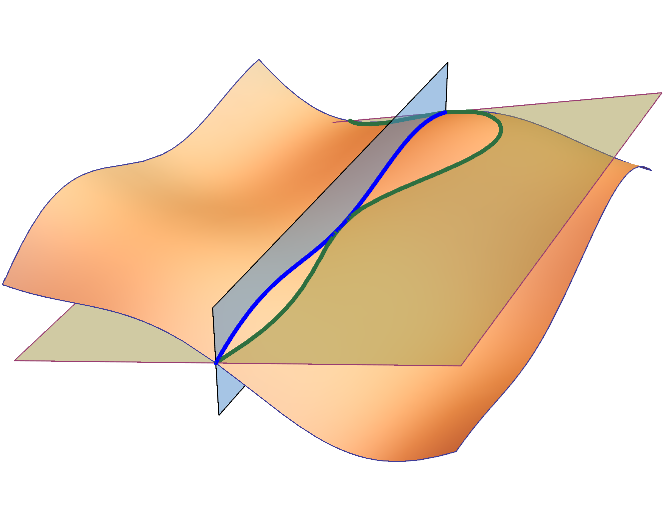
\includegraphics[width=8cm]{./img/ThetaSection.pdf}
	\caption{Нормальное сечение (синим) и сечение\\ наклонённой плоскостью (зелёным)}
\end{figure}

\noindent%
При $\theta = 0$ получаем кривизну нормального сечения:
\begin{equation} \label{eq:NormalCurvature}
	k_n = \pm\frac{\II(\vec{\xi})}{\I(\vec{\xi})}.
\end{equation}
Кривизна сечения под углом $\theta$ теперь выражается через кривизну нормального сечения:
\[
	k_{\theta} = \frac{k_n}{\cos\theta}.
\]
(Обычно теореме Менье формулируют именно в таком виде.)

Формула \ref{eq:NormalCurvature} даёт основной геометрический смысл второй квадратичной формы --- её значение на единичном касательном векторе есть кривизна нормального сечения, порождённого этим вектором. Итак, пусть имеем касательный вектор $\vec{\xi} = \xi^1\vec{\xi}_1 + \xi^2\vec{\xi}_2$, тогда:
\[
	k_{\vec{\xi}} = \frac{\II(\vec{\xi})}{\I(\vec{\xi})} = \frac{\lambda_1(\xi^1)^2 + \lambda_2(\xi^2)^2}{(\xi^1)^2 + (\xi^2)^2} = \lambda_1\cos^2\varphi + \lambda_2\sin^2\varphi,
\]
где $\varphi = \angle(\vec{\xi}, \vec{\xi}_1)$. Таким образом, нами доказана теорема.

\begin{theorem}[Формула Эйлера] \label{theorem:EulerFormula}
	Кривизна нормального сечения, порождённого касательным вектором $\vec{\xi}$, равна
	\[
		\lambda_1\cos^2\varphi + \lambda_2\sin^2\varphi,
	\]
	где $\lambda_1$ и $\lambda_2$ --- главные кривизны, а $\varphi$ --- угол между $\vec{\xi}$ и главным направлением $\vec{\xi}_1$.
\end{theorem}

Положим для определённости $\lambda_1 \leqslant \lambda_2$. Тогда главные кривизны $\lambda_1$ и $\lambda_2$ --- минимум и максимум, соответственно, кривизн нормальных сечений в рассматриваемой точке. (Функция $\lambda_1\cos^2\varphi + \lambda_2\cos^2\varphi$ определена на окружности, а окружность компактна, поэтому максимум и минимум достигаются.) При этом все значения между $\lambda_1$ и $\lambda_2$ достигаются в силу непрерывности. Отметим, что если $\lambda_1\lambda_2 \leqslant 0$, то существует нормальное сечение с нулевой кривизной, то есть прямая.

\begin{corollary}
	$\ds H = \frac{1}{\pi}\int\limits_0^{2\pi}k_{\cos\varphi \cdot \vec{\xi}_1 + \sin\varphi \cdot \vec{\xi}_2}d\varphi$.
\end{corollary}

Средняя кривизна оправдывает своё название не только и даже не столько тем, что является удвоенным средним арифметическим главных кривизн. Она является удвоенным усреднённым значением по \underline{всем} направлениям нормальной кривизны.

\subsection{Минимальные поверхности}

В этом разделе мы рассмотрим один важный класс поверхностей. Для понимания происходящего следует сначала прочитать про деривационные формулы Гаусса "---Вайнгартена.

\begin{definition}
	Гладкая поверхность $\M$ называется \textit{минимальной}, если для любой её внутренней точки $\vec{x}$ найдётся такая окрестность $U$, что любая другая гладкая поверхность $\M^\prime$, совпадающая с $\M$ вне $U$ и имеющая тот же край $\partial\M^\prime = \partial\M$, имеет площадь не меньшую, чем $\M$.
\end{definition}

%Здесь гладкая поверхность понимается в более сильном смысле, чем обычно. Обычно мы считаем, что гладкая поверхность локально является образом гладкого отображения из некоторой области плоскости с наложенным на него условием регулярности. Здесь же предлагается считать, что гладкая поверхность локально является образом гладкого регулярного \underline{гомеоморфизма} из двумерного диска.
%
%Тогда можно сказать, что точка \textit{внутренняя} для поверхности, если при таком гомеоморфизме она соответствует внутренней точке диска. \textit{Краем} поверхности назовём множество её точек, не являющихся внутренними. Корректность этих определений (то есть независимость от выбора конкретного гомеоморфизма) легко проверить.

\begin{theorem}
	Поверхность минимальна тогда и только тогда, когда её средняя кривизна всюду равна нулю.
\end{theorem}

\begin{proof}
	Мы докажем только необходимость условия $H = 0$ для того, чтобы поверхность была минимальна.

	Пусть $\M$ --- минимальная поверхность, $\vec{x}$ --- её внутренняя точка, $\mathcal{N} \subset \M$ --- окрестность точки $\vec{x}$ на поверхности $\M$ такая, что площадь области $\mathcal{N}$ не меньше площади любой другой области с тем же краем.

	Выберем регулярную параметризацию $\vec{r}(u, v)$ на $\mathcal{N}$ и возьмём произвольную гладкую функцию $\varphi\colon \mathcal{N} \to \R$, обращающуюся в нуль вместе со своими производными на крае $\partial\mathcal{N}$, но такую, что $\varphi(\vec{x}) \ne 0$. Рассмотрим следующее семейство параметризованных поверхностей:
	\[
		\vec{r}_t(u, v) = \vec{r}(u, v) + t\varphi(u, v)\vec{n}(u, v),
	\]
	где $\vec{n}$, как обычно, --- вектор нормали. При каждом фиксированном $t$ из достаточно малой окрестности нуля эта формула задаёт регулярную параметризацию некоторой поверхности $\mathcal{N}_t$ с тем же краем, что и $\mathcal{N}$. Так что по построению $\sigma(\mathcal{N}_t) \geqslant \sigma(\mathcal{N})$. Напомним формулу для площади на поверхности:
	\[
		\sigma(\mathcal{N}) = \iint\limits_{\mathcal{N}}\sqrt{\det\G}\,dudv,
	\]
	где $\G$ --- риманова метрика на поверхности $\mathcal{N}$. Для регулярной параметризации подынтегральное выражение гладко зависит от первых производных радиус-вектора $\vec{r}$ по $u$ и $v$, поэтому $\sigma(\mathcal{N}_t)$ --- гладкая функция от $t$. Будем понимать $g(t)$ определитель матрицы первой квадратичной формы поверхности $\mathcal{N}_t$. Далее хотим найти производную $\ds\frac{\partial}{\partial t}\sqrt{g}$.
	\[
		g_{ij}(t) = \langle\vec{r}_i + t(\varphi_i\vec{n} + \varphi\vec{n}_i) + \o(t), \vec{r}_j + t(\varphi_j\vec{n} + \varphi\vec{n}_j) + \o(t)\rangle = \langle\vec{r}_i + t\varphi\vec{n}_i, \vec{r}_j + t\varphi\vec{n}_j\rangle + \o(t)
	\]
	при $t \to 0$, поскольку $\vec{n} \perp \vec{r}_k$, $k = 1, 2$. Таким образом, $g(t)$ с точностью до $\o(t)$ есть матрица Грама векторов $\vec{r}_1 + t\varphi\vec{n}_1$, $\vec{r}_2 + t\varphi\vec{n}_2$, и выражается через них матрицей
	\[
		E + t\varphi C,
	\]
	где $C = -\G^{-1}\B$ --- матрица оператора Вайнгартена. (Это сразу следует из деривационных формул Вайнгартена.) Далее, вместо того, чтобы непосредственно вычислять $\sqrt{g(t)}$, вспомним, что эта величина равна площади параллелограмма, натянутого на соответствующую пару векторов, а отношение площадей равно абсолютной величине определителя соответствующей матрицы перехода, откуда
	\[
		\frac{\sqrt{g(t)}}{\sqrt{g(0)}} = \abs{\det(E + t\varphi C)} + \o(t) = 1 + t\varphi\tr C + \o(t) = 1 + t\varphi H + \o(t)
	\]
	как следствие теоремы \ref{theorem:Weingarten}. Отсюда получаем $g^\prime = \sqrt{\det \G}\varphi H$. Таким образом,
	\[
		\sigma(\mathcal{N}_t) = \sigma(\mathcal{N}) + t\iint\limits_{\mathcal{N}}\sqrt{\det \G}\varphi H\,dudv + \o(t).
	\]
	Посколько площадь поверхности $\mathcal{N}_t$ достигает минимума при $t = 0$ мы должны иметь
	\[
		0 = \left.\frac{d\sigma(\mathcal{N}_t)}{dt}\right|_{t = 0} = \iint\limits_{\mathcal{N}}\sqrt{\det \G}\varphi H\,dudv
	\]
	при любом выборе функции $\varphi$. Покажем, что неравенство $H \ne 0$ ведёт к противоречию с этим условием. Возьмём новую функцию $\widetilde{\varphi} = \varphi^2H$. Получим
	\[
		\iint\limits_{\mathcal{N}}\sqrt{\det \G}\widetilde{\varphi}H\,dudv = \iint\limits_{\mathcal{N}}\sqrt{\det\G}\varphi^2H^2\,dudv > 0,
	\]
	так как подынтегральная функция неотрицательна, причём в точке $\vec{x}$ она положительна.
\end{proof}

Физический смысл минимальных поверхностей следующий. Если между двумя кривыми в пространстве натянуть мыльную плёнку, то она, стремясь всюду локально уменьшить свою площадь, примет форму минимальной поверхности. Самые простые примеры минимальных поверхностей --- плоскость, геликоид и катеноид (на геликоид и катеноид можно посмотреть на рисунке \ref{fig:HelicoidCatenoid}). В этом легко убедиться, посчитав их среднюю кривизну.

%\begin{figure}[H]
%	\centering
%	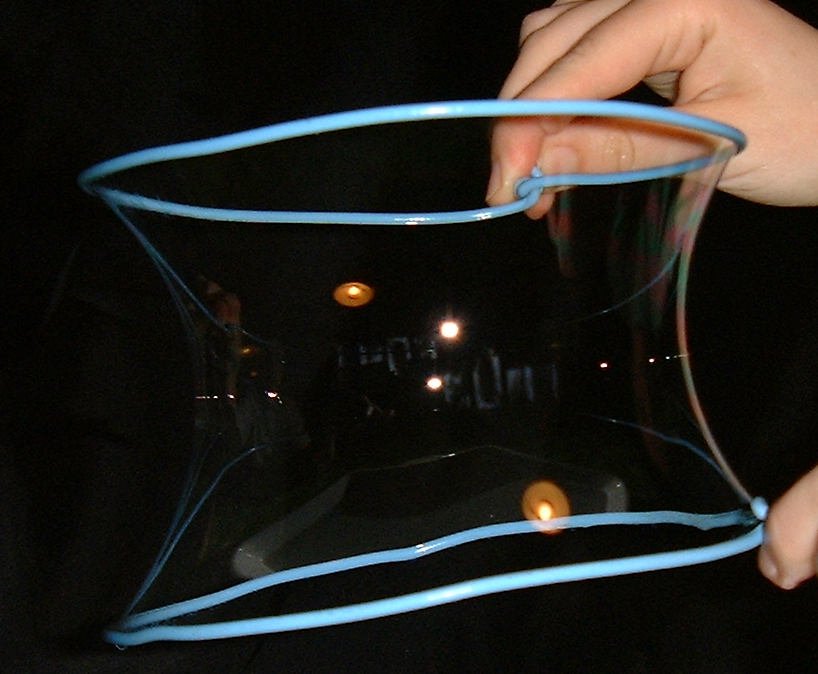
\includegraphics[width=6cm]{./img/Membrane.png}
%	\caption{Мыльная плёнка в форме катеноида}
%\end{figure}

% TODO: нахождение омбилических точек (к примеру, у эллипсоида)

% TODO: Дописать про эпиграф

